% Manuscrito de tesis. Compilar desde informe/:
%   ../.venv/Scripts/python.exe tablas_manuscrito.py
%   ./tectonic.exe tesis.tex
\documentclass[12pt,a4paper,oneside]{report}
\usepackage{fontspec}
\usepackage[spanish,es-nodecimaldot,es-noshorthands,es-tabla]{babel}
\addto\captionsspanish{\renewcommand{\bibname}{Referencias}}
\usepackage[left=3cm,right=2.5cm,top=2.5cm,bottom=2.5cm]{geometry}
\usepackage{setspace}
\usepackage{amsmath,amssymb}
\usepackage{graphicx}
\usepackage{booktabs,array,tabularx,longtable}
\usepackage{float}
\usepackage[font=small,labelfont=bf]{caption}
\usepackage{xcolor}
\usepackage[round,authoryear]{natbib}
\usepackage{enumitem}
\usepackage[hidelinks]{hyperref}
\usepackage{xurl}

\graphicspath{{../notebooks/resultados/figuras/}}
\onehalfspacing
\setlength{\parskip}{0.35em}
\setlength{\emergencystretch}{3em}
\newcommand{\origen}[1]{\par\vspace{2pt}{\raggedright\footnotesize\textit{Fuente:} #1\par}}
\newcommand{\pendiente}[1]{\textcolor{red}{[#1]}}

\begin{document}

% ------------------------------------------------------------------ portada
\begin{titlepage}
\centering
{\large \pendiente{UNIVERSIDAD}\par}
{\large \pendiente{FACULTAD}\par}
{\large \pendiente{ESCUELA PROFESIONAL}\par}
\vspace{2.5cm}
{\Large\bfseries INFERENCIA CAUSAL ESPACIAL ASISTIDA POR INTELIGENCIA ARTIFICIAL PARA LA VALORACIÓN CONTRAFACTUAL DE ATRIBUTOS RESIDENCIALES: EL EFECTO DE LA COCHERA INCLUIDA EN EL PRECIO DE OFERTA DE ALQUILER EN LIMA METROPOLITANA\par}
\vspace{2cm}
{\large TESIS\par}
{\large Para optar el título profesional de \pendiente{título}\par}
\vspace{1.5cm}
{\large Elaborada por\par}
{\large\bfseries Luis Azaña\par}
\vspace{1cm}
{\large Asesor\par}
{\large \pendiente{Nombre del asesor}\par}
\vfill
{\large Lima, Perú\par}
{\large 2026\par}
\end{titlepage}

\pagenumbering{roman}

% ------------------------------------------------------------------ resumen
\chapter*{Resumen}
\addcontentsline{toc}{chapter}{Resumen}
Esta tesis estima el efecto causal de que un departamento en alquiler incluya cochera sobre su precio de oferta en Lima Metropolitana. A diferencia de los trabajos locales previos, que predicen precios, el objetivo es separar la asociación hedónica del efecto atribuible al atributo bajo supuestos explícitos. Se auditaron 3\,739 avisos obtenidos por \textit{web scraping} en 13 distritos (marzo de 2025): se eliminaron 243 duplicados (83 de ellos, el mismo aviso registrado en dos distritos) y se conservaron solo las direcciones geocodificadas con precisión exacta (\texttt{ROOFTOP}), con lo que la muestra queda en 2\,220 avisos. La disponibilidad de cochera no figuraba en los datos: se extrajo del texto de cada aviso combinando un filtro con expresiones regulares y un modelo de lenguaje (\texttt{gpt-4.1-mini}, salida JSON con esquema fijo), con un costo total de 0.76 USD. Un grafo acíclico dirigido justifica el conjunto de ajuste: área, dormitorios, baños, antigüedad, ubicación, días publicado y tipo de geocodificación. El estimador principal es Double Machine Learning interactivo (IRM/AIPW), con \textit{cross-fitting} agrupado por edificio, errores estándar agrupados y recorte al soporte común (propensión entre 0.05 y 0.95; 1\,949 avisos). La diferencia bruta es del 63\,\%; el efecto estimado es de \textbf{7.5\,\% (IC 95\,\%: 3.7--11.4\,\%)}, unos S/\,199 mensuales sobre un alquiler de referencia de S/\,2\,650. El efecto es heterogéneo: casi nulo en los distritos de mayor precio (1.5\,\%) y mayor donde las cocheras son escasas (10\,\% y 18\,\%; Wald, $p<0.001$). Como análisis secundario, un baño adicional eleva el precio en 3.8\,\% (1.7--6.0\,\%). Ambos resultados son moderadamente frágiles: un confusor omitido tan fuerte como la antigüedad los llevaría cerca de cero. Una validación semisintética con 800 réplicas muestra que los estimadores recuperan el efecto cuando no hay confusión omitida, pero que la cota de sensibilidad del estimador binario es optimista. Los resultados son causales solo de forma condicional a los supuestos, válidos para la población de avisos publicados y exploratorios mientras la extracción con IA no se valide con etiquetas humanas.

\noindent\textbf{Palabras clave:} inferencia causal; Double Machine Learning; precios hedónicos; alquiler; cochera; modelos de lenguaje; análisis de sensibilidad; Lima.

\chapter*{Abstract}
\addcontentsline{toc}{chapter}{Abstract}
This thesis estimates the causal effect of an included parking space on the asking rent of apartments in Metropolitan Lima. Unlike previous local studies, which predict prices, the goal is to separate hedonic association from the effect attributable to the attribute under explicit assumptions. We audited 3,739 web-scraped listings from 13 districts (March 2025), removed 243 duplicates (83 of them the same listing recorded under two districts) and kept only exactly geocoded addresses (\texttt{ROOFTOP}), leaving 2,220 listings. Parking availability was not a structured field: it was extracted from each listing's text with a regular-expression filter followed by a language model (\texttt{gpt-4.1-mini}, fixed JSON schema), at a total cost of USD 0.76. A directed acyclic graph justifies the adjustment set: floor area, bedrooms, bathrooms, building age, location, days on market and geocoding type. The main estimator is an interactive Double Machine Learning model (IRM/AIPW) with building-grouped cross-fitting, cluster-robust standard errors and trimming to the common-support population (propensity between 0.05 and 0.95; 1,949 listings). The raw difference is 63\%; the estimated effect is \textbf{7.5\% (95\% CI: 3.7--11.4\%)}, about PEN 199 per month for a reference rent of PEN 2,650. The effect is heterogeneous: almost zero in the most expensive districts (1.5\%) and larger where parking is scarce (10\% and 18\%; Wald $p<0.001$). As a secondary analysis, an additional bathroom raises rent by 3.8\% (1.7--6.0\%). Both results are moderately fragile: an omitted confounder as strong as building age would bring them close to zero. A semi-synthetic validation with 800 replications shows that the estimators recover the effect without omitted confounding, but that the sensitivity bound of the binary estimator is optimistic. The findings are causal only conditionally on the stated assumptions, apply to published listings, and remain exploratory until the AI extraction is validated against human labels.

\noindent\textbf{Keywords:} causal inference; double machine learning; hedonic pricing; rental housing; parking; large language models; sensitivity analysis; Lima.

\tableofcontents
\listoftables
\listoffigures

\clearpage
\pagenumbering{arabic}

\chapter{Introducción}

\section{Contexto}

El alquiler es una vía de acceso a la vivienda cada vez más importante en Lima Metropolitana. En los distritos consolidados del centro y del sur de la ciudad, la oferta de departamentos se publica sobre todo en portales inmobiliarios, donde cada aviso informa el precio pedido y un conjunto de atributos: área, número de dormitorios y de baños, antigüedad del edificio, ubicación y una descripción libre. Esa información permite estudiar con un nivel de detalle inédito cómo se forma el precio de oferta.

La literatura peruana sobre el tema ha seguido dos caminos. El primero es el enfoque hedónico clásico, que interpreta los coeficientes de una regresión del precio sobre los atributos como ``precios implícitos'' de cada característica \citep{rosen1974}. El índice hedónico de precios de departamentos del Banco Central de Reserva del Perú encuentra, por ejemplo, que el número de cocheras y el número de baños están entre las características más valoradas en Lima \citep{mundaca2018}. El segundo camino, más reciente, aplica aprendizaje automático para \emph{predecir} precios de venta o de alquiler \citep{cacnahuaray2024,barrientos2026}. Ambos son útiles, pero ninguno responde una pregunta contrafactual: \emph{¿cuánto cambiaría el precio de un departamento si tuviera un baño más, sin cambiar nada de lo demás?}

\section{Problema}

La respuesta a esa pregunta no se puede leer en una correlación ni en un coeficiente predictivo. Los departamentos con más baños son, en promedio, más grandes, más nuevos y están mejor ubicados; cada una de esas características también eleva el precio. En los datos de esta tesis, un baño adicional se asocia con un precio 45\,\% mayor cuando no se ajusta por nada, cifra que confunde el efecto del baño con el del tamaño y la zona. Al ajustar, aparece un segundo problema: ¿por qué variables ajustar? Agregar todas las disponibles no es inocuo. Algunas, como el precio por metro cuadrado, son consecuencia del precio y destruyen la estimación; otras, como los dormitorios, se deciden junto con los baños al diseñar el plano. Y queda un tercer problema que ningún ajuste resuelve: atributos no observados, como la calidad de los acabados, el piso o la vista, pueden influir tanto en el número de baños como en el precio.

El aprendizaje automático causal, en particular \textit{Double/Debiased Machine Learning} \citep{chernozhukov2018}, permite ajustar por muchas variables de forma flexible sin imponer una forma funcional y conservar una inferencia válida. Pero la flexibilidad del estimador no sustituye la estrategia de identificación \citep{hunermund2023}. La contribución de esta tesis es aplicar ese marco a un atributo residencial concreto en Lima, haciendo explícitos los supuestos, auditando los datos y midiendo cuán frágil es la conclusión.

\section{Pregunta de investigación}

\begin{quote}
¿En qué medida un diseño de aprendizaje causal con ajuste espacial permite estimar, dentro de la población de avisos comparables, la prima contrafactual sobre el precio de oferta de alquiler asociada a un baño adicional, y cuán estable es esa estimación frente a confusión no observada y a las decisiones de modelado?
\end{quote}

\section{Objetivos}

\subsection{Objetivo general}
Estimar y evaluar la robustez del efecto causal de un baño adicional sobre el precio de oferta del alquiler de departamentos en Lima Metropolitana. Para ello se usan métodos de aprendizaje causal ortogonal, controles espacialmente informados e inferencia que respeta la dependencia entre avisos.

\subsection{Objetivos específicos}
\begin{enumerate}[label=\textbf{OE\arabic*.}, leftmargin=*]
  \item Auditar, depurar y caracterizar los avisos y la selección de la muestra (procedencia, duplicados, exclusiones y perfil territorial).
  \item Definir la intervención y justificar su identificación (estimando, DAG, conjunto de ajuste, población y amenazas no identificables).
  \item Estimar y comparar la asociación hedónica con el ML causal (efecto principal con IC 95\,\%, diagnósticos de los modelos auxiliares y comparación de estimadores).
  \item Evaluar la variación socioespacial y la sensibilidad de los resultados (efectos por grupos, grilla de especificaciones, confusión no observada y dependencia espacial).
  \item Cuantificar el aporte de atributos medidos mediante IA a partir del texto de los avisos. \textit{En este entregable no se ejecuta}: la sección~\ref{sec:oe5} justifica la decisión y deja el diseño preparado.
  \item Verificar el comportamiento del procedimiento con una verdad conocida (validación semisintética: sesgo, RMSE y cobertura).
  \item Garantizar la trazabilidad de los resultados: cada tabla y figura indica el notebook y el archivo que la generan.
\end{enumerate}

\section{Hipótesis}

Las hipótesis no exigen por anticipado un efecto significativo ni positivo:
\begin{description}[leftmargin=1.2cm]
  \item[H1.] La magnitud de la asociación inicial cambia de forma mensurable tras el ajuste preespecificado.
  \item[H2.] La omisión de confusores o la inclusión de controles causalmente inadecuados altera la estimación más que la elección del algoritmo de predicción.
  \item[H3.] Existe heterogeneidad del efecto según el contexto territorial o el tamaño del departamento, y solo se afirmará si la precisión estadística la respalda.
  \item[H4.] La solidez de la conclusión depende de la fuerza que se postule para los confusores no observados.
\end{description}

\section{Alcance y aportes}

\textbf{Alcance.} El objeto son los precios \emph{de oferta} mensuales de departamentos publicados en un portal, no contratos firmados ni el bienestar de los hogares. La cobertura son 13 distritos de Lima Metropolitana con avisos activos en marzo de 2025. La unidad de análisis es el aviso, con un manejo explícito de los avisos repetidos y de la agrupación por edificio y por zona. Los resultados no se extrapolan al parque residencial completo ni a otros distritos.

\textbf{Aportes verificables.} (i) Una auditoría reproducible de la base, que documenta duplicados entre distritos y errores de geocodificación que no se habían detectado. (ii) Una estimación del efecto de un baño adicional con identificación explícita, inferencia agrupada y comparación con el enfoque hedónico. (iii) Una demostración empírica de cómo la elección de controles cambia el resultado. (iv) Un análisis de sensibilidad calibrado con confusores observados. (v) Una validación semisintética anclada en las covariables reales del mercado limeño.

\textbf{Limitaciones principales.} El tratamiento no se asignó al azar, por lo que la interpretación causal depende de la ausencia de confusores omitidos importantes, supuesto que solo puede acotarse. La muestra corresponde a un único corte de un portal, y la antigüedad falta en el 25\,\% de la muestra final. Los atributos de calidad del texto aún no se extraen (OE5).

\section{Organización del documento}

El capítulo~\ref{cap:estado} revisa la literatura. El capítulo~\ref{cap:marco} presenta el modelo causal, el estimando y el DAG. El capítulo~\ref{cap:datos} describe los datos, la auditoría y los métodos de estimación, y el capítulo~\ref{cap:diseno} el diseño de las pruebas de robustez y de la validación semisintética. El capítulo~\ref{cap:resultados} reporta los resultados, el~\ref{cap:discusion} los discute y el~\ref{cap:conclusiones} presenta las conclusiones por objetivo. Los anexos contienen el diccionario de variables, el registro de la búsqueda bibliográfica, el inventario de artefactos y las versiones de software.

\chapter{Antecedentes y estado del arte}\label{cap:estado}

Este capítulo resume una revisión focalizada y documentada, no una revisión sistemática PRISMA. Las cadenas de búsqueda, las fuentes y los criterios están en el anexo~\ref{anx:busqueda}. Se organiza en cinco frentes, del más cercano al más general:
\begin{enumerate}[label=(\roman*)]
\item los antecedentes peruanos sobre el precio de la vivienda;
\item la cochera como atributo residencial y su contexto en Lima;
\item el paso del aprendizaje automático predictivo al causal;
\item el uso de avisos en línea y de su texto como fuente de datos;
\item la síntesis y el vacío que aborda esta tesis.
\end{enumerate}
Las afirmaciones de originalidad se limitan a las fuentes consultadas.

\section{Marco de referencia: precios hedónicos}

\citet{rosen1974} formalizó la idea de que el precio de un bien diferenciado depende de sus atributos y de que la derivada de esa función respecto de un atributo es su precio implícito. El modelo hedónico se convirtió en la herramienta estándar para valorar atributos de la vivienda \citep{malpezzi2003}. La revisión de \citet{sirmans2005} muestra, sin embargo, que el coeficiente de un mismo atributo varía mucho entre estudios según qué otras variables se controlen. Un precio implícito es \emph{condicional a la especificación}: no indica por sí mismo cuánto cambiaría el precio si se modificara el atributo. Esa distinción entre asociación y efecto organiza todo el capítulo.

\section{Antecedentes peruanos}\label{sec:peru}

\paragraph{Índices hedónicos.} \citet{mundaca2018}, del BCRP, construyen un índice de precios de departamentos \emph{en venta} para diez distritos de Lima (unos 30\,000 avisos, 2008--2016). En sus regresiones semilogarítmicas, el número de cocheras y el de baños son las características con mayor valoración por unidad. Su objetivo es el índice, no identificar efectos. Los propios autores reportan variables omitidas en sus modelos y señalan como principal limitación la falta de un buen indicador de ubicación. \citet{mayo2017} elabora en la Universidad Nacional de Ingeniería un índice hedónico de viviendas \emph{nuevas} con datos del Fondo MiVivienda (2001--2015), y \citet{rivera2018} estudia los determinantes del precio por metro cuadrado (2005--2017). Los tres trabajan con precios de venta y modelos lineales.

\paragraph{Aprendizaje automático predictivo.} \citet{cacnahuaray2024} predicen el alquiler de departamentos en la provincia de Lima con 3\,675 avisos de 2023 y técnicas de AutoML. Entre los predictores más importantes que reportan están el área y el número de cocheras. \citet{barrientos2026} comparan árboles de decisión y XGBoost con la regresión hedónica sobre más de 40\,000 registros del BCRP (2014--2024) e identifican el tamaño, la cochera y la ubicación como los determinantes principales. Ambos confirman que la cochera es relevante para \emph{predecir} el precio en Lima, pero no estiman cuánto lo cambia.

\paragraph{Inferencia causal sobre vivienda en Lima.} El único antecedente local con una estrategia de identificación explícita es \citet{contreras2024}. Con diferencias en diferencias, aprovechan la apertura escalonada de la Línea 1 del Metro para estimar su efecto sobre la informalidad de la vivienda. Su variable de interés no es el precio, pero muestra que el razonamiento causal ya se aplica a la vivienda limeña.

\section{La cochera como atributo residencial}\label{sec:cochera_lit}

\paragraph{Evidencia sobre su valor en alquileres.} La referencia más directa por el tipo de tratamiento es \citet{gabbe2017}. Con más de 38\,000 viviendas en alquiler de áreas metropolitanas de Estados Unidos, estiman que una cochera incluida en el alquiler eleva la renta en alrededor de 17\,\%. \citet{manville2013} encuentra en Los Ángeles que la cochera incluida añade unos 200 dólares mensuales al alquiler. Ambos estudian mercados con una tenencia de automóviles muy superior a la de Lima, por lo que sirven para contrastar la dirección y el orden de magnitud, no para comparar cifras directamente.

\paragraph{Contexto limeño.} Tres hechos locales son relevantes para interpretar el valor de la cochera en Lima:
\begin{itemize}[leftmargin=*]
\item \textbf{Regulación.} En los distritos centrales, la normativa municipal fija un número mínimo de estacionamientos por unidad de vivienda: Miraflores lo hace en el artículo 10 de la Ordenanza 342-MM \citep{miraflores2011} y San Isidro en la Ordenanza 523-MSI \citep{sanisidro2020}. Ahí la cochera tiende a ser un componente estándar de los edificios nuevos.
\item \textbf{Mercado.} El índice de referencia del mercado de alquiler, que también usa el BCRP, toma como unidad típica un departamento de 60 o 100\,m² \emph{con un estacionamiento} \citep{urbania2025}.
\item \textbf{Demanda.} Solo alrededor del 17\,\% de los hogares de Lima y Callao tenía al menos un automóvil en 2015 \citep{limacomovamos2016}, frente a una mayoría en los mercados estadounidenses citados.
\end{itemize}
Estos hechos sugieren que el valor de la cochera en Lima debería ser menor que en Estados Unidos y distinto según la zona. Esta tesis lo pone a prueba.

\section{Del aprendizaje automático predictivo al causal}

\paragraph{Predicción.} Además de los estudios peruanos, la literatura internacional usa el aprendizaje automático para valuar inmuebles. \citet{tapia2025} comparan modelos automáticos de valuación con hedónicos espaciales en Santiago de Chile. \citet{gyger2026} combinan un proceso gaussiano espacial con \textit{tree boosting} para modelar alquileres en Alemania. Estos trabajos mejoran la predicción, pero las importancias de variables o los valores SHAP describen cómo usa el modelo cada variable, no el efecto de intervenirla.

\paragraph{Identificación causal en vivienda.} La economía urbana estima el valor de amenidades con diseños cuasiexperimentales, como discontinuidades en fronteras \citep{black1999,keele2015} o cambios regulatorios \citep{chay2005}. Cuando no hay una fuente de variación casi aleatoria, como ocurre con la cochera de un departamento, la alternativa es ajustar por los confusores observados bajo ignorabilidad condicional y acotar el sesgo por confusores omitidos.

\paragraph{Double Machine Learning.} \citet{chernozhukov2018} muestran que, si se estiman las funciones auxiliares con aprendizaje automático, se ortogonaliza el problema y se usa \textit{cross-fitting}, el efecto es consistente y admite inferencia válida. Para tratamientos binarios, la versión interactiva (IRM/AIPW) es doblemente robusta. El marco tiene limitaciones conocidas. \citet{hunermund2023} muestran que DML es muy sensible a la inclusión de malos controles, y \citet{cinelli2024} sistematizan qué variables deben y no deben ajustarse. \citet{wager2018} y \citet{athey2019} extienden el enfoque a efectos heterogéneos, cuya estimación es frágil en muestras moderadas \citep{knaus2021}.

\paragraph{Robustez y validación.} \citet{cinelli2020} y \citet{chernozhukov2022} formulan cotas de sesgo por confusores omitidos que se calibran con confusores observados. \citet{moran1950} y \citet{cameron2015} proveen herramientas para la dependencia espacial y la inferencia agrupada. \citet{advani2019} recomiendan validar los estimadores con simulaciones ancladas en los datos reales, y \citet{chen2026} lo hacen al comparar regresiones hedónicas y aprendizaje causal en vivienda.

\section{Avisos en línea y su texto como fuente de datos}

\paragraph{Avisos como datos.} \citet{boeing2017} muestran que los avisos de alquiler extraídos por \textit{web scraping} permiten estudiar mercados de alquiler a gran escala. También advierten que exigen limpieza, deduplicación y cuidado al interpretarlos como precios de oferta.

\paragraph{Información en el texto.} \citet{nowak2017} encuentran que el texto libre de los avisos reduce en más de 25\,\% el error de precio de un modelo hedónico, y \citet{shen2021} que la información ``blanda'' de la descripción tiene un valor significativo en el precio. Los atributos relevantes no siempre están en los campos estructurados.

\paragraph{Modelos de lenguaje para medir atributos.} \citet{faxvaag2026} usan modelos GPT para extraer de los avisos de Oslo variables cuantitativas, entre ellas el estacionamiento, e incorporarlas a un modelo de valuación. Es el precedente metodológico más cercano a la medición de la cochera de esta tesis. \citet{egami2023} advierten que usar etiquetas producidas por un modelo de lenguaje directamente en un análisis estadístico produce sesgo e intervalos inválidos, incluso con un 80--90\,\% de acierto. Proponen combinarlas con una muestra etiquetada por personas mediante un estimador doblemente robusto, lo que justifica la validación humana prevista en esta tesis.

\section{Síntesis y vacío}

\begin{table}[H]
\centering\small
\caption{Cuadro comparativo de antecedentes}\label{tab:comparativo}
\begin{tabularx}{\textwidth}{>{\raggedright\arraybackslash}p{2.6cm}>{\raggedright\arraybackslash}p{2.5cm}>{\raggedright\arraybackslash}X>{\raggedright\arraybackslash}p{2.6cm}}
\toprule
Trabajo & Objeto / datos & Qué aporta y límite & Método \\
\midrule
\citet{mundaca2018} & Venta, Lima, 2008--2016 & Cochera y baños, lo más valorado; asociativo, ubicación por distrito & Hedónico \\
\citet{mayo2017}; \citet{rivera2018} & Venta, Lima & Índice y determinantes del precio/m²; asociativo & Hedónico / regresión \\
\citet{cacnahuaray2024} & Alquiler, Lima, 2023 & La cochera, entre los predictores más fuertes; no estima efecto & ML predictivo \\
\citet{barrientos2026} & Venta, Lima (BCRP) & La cochera como determinante clave; predictivo & XGBoost vs. hedónico \\
\citet{contreras2024} & Informalidad, Lima & Único causal local; no estudia precios & Diferencias en diferencias \\
\citet{gabbe2017} & Alquiler, EE.\,UU. & Cochera incluida +17\,\% del alquiler; otro mercado & Hedónico \\
\citet{faxvaag2026} & Avisos, Oslo & Estacionamiento extraído con GPT; objetivo predictivo & LLM + valuación \\
\citet{egami2023} & Metodológico & Uso válido de etiquetas de LLM con validación humana & DSL (doblemente robusto) \\
\textbf{Esta tesis} & \textbf{Alquiler, Lima, 2025} & \textbf{Efecto causal de la cochera medida con IA, con soporte común y sensibilidad} & \textbf{DML-IRM + validación semisintética} \\
\bottomrule
\end{tabularx}
\end{table}

La tabla~\ref{tab:comparativo} resume la posición de la tesis. Los estudios peruanos coinciden en que la cochera es un atributo relevante del precio, pero la abordan con modelos asociativos o predictivos y sobre precios de venta. La literatura internacional ofrece evidencia sobre el valor de la cochera en alquileres y herramientas para estimar efectos causales y medir atributos desde el texto. En las fuentes consultadas no se encontró un estudio sobre Lima que combine las tres piezas: estimar causalmente el valor de un atributo del alquiler, medir ese atributo desde el texto con IA y acotar la fragilidad del resultado. Ese es el espacio en que se sitúa esta tesis.

\chapter{Fundamentos y modelo causal}\label{cap:marco}

\section{Resultados potenciales y estimando}

Sea $i$ un aviso de alquiler y $D_i\in\{0,1\}$ el tratamiento: $D_i=1$ si el departamento incluye cochera en el alquiler y $D_i=0$ si no tiene cochera. El resultado es $Y_i=\ln P_i$, el logaritmo del precio mensual de oferta. En el lenguaje de resultados potenciales \citep{imbens2015,hernan2020}, $Y_i(1)$ y $Y_i(0)$ son los log-precios que se pedirían por el mismo departamento con y sin cochera incluida, con el resto de sus atributos fijos. El estimando principal es el efecto promedio del tratamiento en la población con soporte común:
\begin{equation}\label{eq:ate}
\theta = E\big[\,Y(1)-Y(0)\;\big|\;X\in\mathcal{S}\,\big],\qquad \mathcal{S}=\{x:\;0.05\le m(x)\le0.95\},
\end{equation}
donde $m(x)=P(D=1\mid X=x)$ es la propensión. El efecto en porcentaje es $100\,(e^\theta-1)$. En soles se reporta solo para un alquiler de referencia fijado de antemano: la mediana de la muestra (S/\,2\,650).

La restricción a $\mathcal{S}$ es deliberada. Para un departamento cuyo perfil hace casi seguro que tenga cochera (o que no la tenga), los datos no contienen comparaciones creíbles, y el efecto en ese perfil solo podría obtenerse extrapolando. Recortar cambia la población a la que se refiere el resultado; por eso se reporta también el efecto sin recorte.

\paragraph{Tratamiento secundario.} Para el número de baños $T\in\{1,\dots,5\}$, un conteo, el estimando es el coeficiente $\theta_T$ del modelo parcialmente lineal \citep{robinson1988}:
\begin{equation}\label{eq:plr}
Y = \theta_T\,T + g(X) + \varepsilon,\qquad T = m_T(X) + V,
\end{equation}
interpretado como el efecto medio de un baño adicional, ponderado por la varianza condicional de $T$.

\section{Supuestos de identificación}

\begin{enumerate}[leftmargin=*]
\item \textbf{Ignorabilidad condicional.} $Y(1),Y(0)\perp D\mid X$: entre departamentos iguales en $X$, que uno tenga cochera no depende de su precio potencial. Se viola si un factor omitido (por ejemplo, la calidad del edificio) afecta a la vez la cochera y el precio.
\item \textbf{Positividad (soporte común).} $0<m(X)<1$. Se diagnostica con la distribución de la propensión por brazo y se impone con el recorte $[0.05,0.95]$.
\item \textbf{Consistencia y versiones del tratamiento.} ``Cochera incluida'' agrupa una o más cocheras, techadas o no. Los avisos con cochera de \emph{costo extra} son otra versión del tratamiento (el precio no la incluye) y se excluyen del análisis principal.
\item \textbf{Medición del tratamiento.} $D$ se mide desde el texto. Se supone que un aviso que no menciona cochera no la tiene. Un error de clasificación no diferencial tiende a atenuar el efecto; uno diferencial puede sesgarlo en cualquier dirección.
\item \textbf{Ausencia de interferencia.} La cochera de un departamento no afecta el precio de otro. Los choques comunes de edificio o de zona se tratan con inferencia agrupada.
\end{enumerate}

\section{Grafo causal (DAG)}

\begin{figure}[H]
\centering
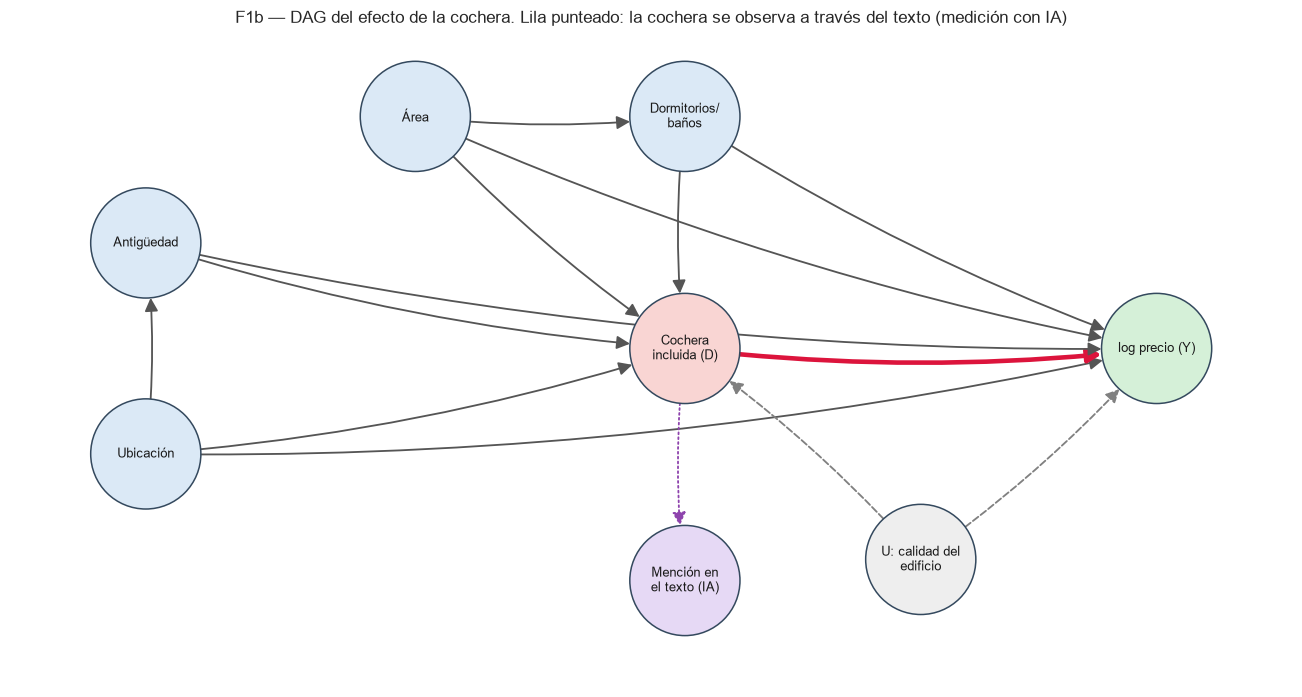
\includegraphics[width=0.95\textwidth]{F1b_dag_cochera.png}
\caption{DAG del efecto de la cochera (F1b). Azul: confusores ajustados; gris punteado: confusor no observado $U$; lila punteado: la cochera se observa a través del texto del aviso.}\label{fig:dag}
\origen{\texttt{notebook3b\_efecto\_cochera.ipynb}, sección 1 $\rightarrow$ \texttt{F1b\_dag\_cochera.png}.}
\end{figure}

La figura~\ref{fig:dag} presenta el modelo causal supuesto, construido con conocimiento del dominio y con el orden temporal de las decisiones. La ubicación y la época de construcción del edificio preceden al diseño. El área, los dormitorios, los baños y la dotación de cocheras se definen en el proyecto. El precio se fija al publicar. Por el criterio \textit{back-door} \citep{pearl2009}, el \textbf{conjunto de ajuste} es: log del área, dormitorios, baños, antigüedad (con un indicador de faltante), latitud, longitud, días publicado, distrito y tipo de lugar devuelto por el geocodificador. El camino $D\leftarrow U\rightarrow Y$ no puede bloquearse con los datos; es la amenaza principal.

Para los baños (análisis secundario) se usa el DAG del entregable anterior (figura~\ref{fig:dag_banos}). Su conjunto de ajuste es el mismo sin los baños; la cochera se agrega como control en una especificación alternativa.

\begin{figure}[H]
\centering
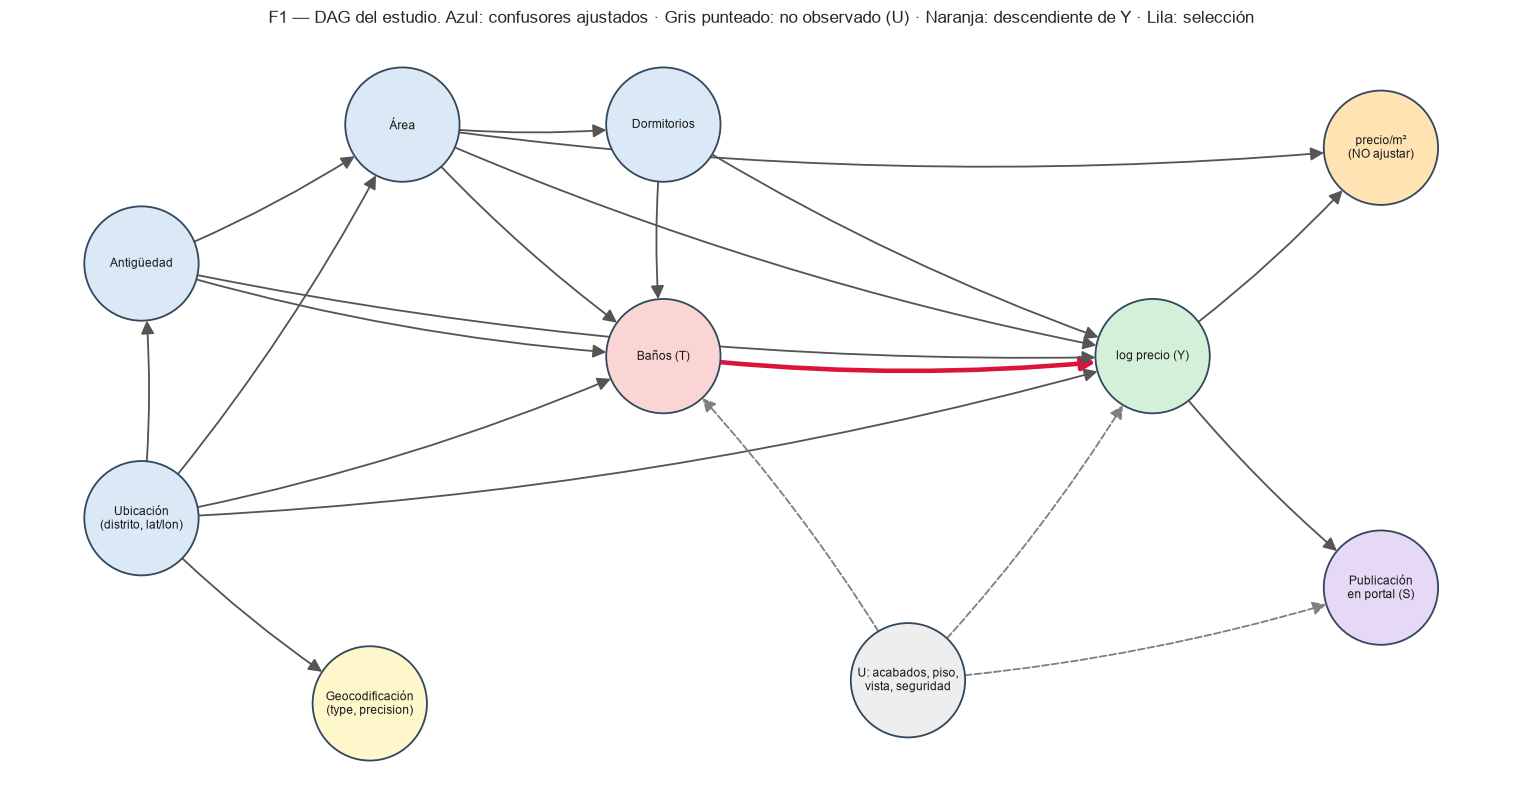
\includegraphics[width=0.85\textwidth]{F1_dag.png}
\caption{DAG del análisis secundario: efecto de un baño adicional (F1).}\label{fig:dag_banos}
\origen{\texttt{notebook3\_estimacion\_causal.ipynb}, sección 1 $\rightarrow$ \texttt{F1\_dag.png}.}
\end{figure}

\section{Papel de cada variable: buenos y malos controles}

\begin{table}[H]
\centering\small
\caption{Papel de cada variable respecto del efecto de la cochera sobre el precio}\label{tab:roles}
\begin{tabularx}{\textwidth}{>{\raggedright\arraybackslash}p{3.0cm}>{\raggedright\arraybackslash}p{2.4cm}>{\raggedright\arraybackslash}p{2.4cm}X}
\toprule
Variable & Papel & ¿Ajustar? & Justificación \\
\midrule
Ubicación (distrito, lat., lon.) & Confusor & Sí & Precede al proyecto; define la escasez de cocheras y el precio \\
Área & Confusor & Sí & Departamentos grandes suelen venir con cochera y cuestan más \\
Baños y dormitorios & Confusores & Sí & Reflejan el estándar del proyecto; no son consecuencia de la cochera \\
Antigüedad & Confusor & Sí & Los edificios antiguos tienen menos cocheras y distinto precio \\
Días publicado, tipo de geocodificación & Previas / artefacto & Sí & Absorben diferencias del aviso y error de ubicación \\
Precio por m² & Descendiente de $Y$ & \textbf{No} & Es el resultado dividido por el área \\
Mención de cochera en el texto & Medición de $D$ & -- & Define el tratamiento; su error es una amenaza \\
Calidad del edificio, amenidades & Confusor no observado $U$ & Imposible & Amenaza principal; se acota con análisis de sensibilidad \\
Publicación en el portal & Selección & Por diseño & Los resultados valen para avisos publicados \\
\bottomrule
\end{tabularx}
\end{table}

\section{Selección, causalidad espacial y amenazas a la validez}

\paragraph{Selección.} La muestra contiene solo departamentos publicados, vigentes en la fecha de captura y con dirección geocodificada con exactitud. Las direcciones exactas son algo más caras y se concentran en los distritos de mayor precio. Por eso los resultados valen para esa población y no se transportan al parque residencial ni a los precios de contrato.

\paragraph{Dependencia espacial.} Departamentos cercanos comparten entorno y los avisos de un mismo edificio comparten su calidad. El \textit{cross-fitting} se agrupa por edificio, los errores estándar se agrupan por edificio (y, como alternativa, por bloques de 1\,km) y la autocorrelación residual se mide con el I de Moran.

\paragraph{Amenazas.} (i) Confusores no observados de calidad. (ii) Error de medición del tratamiento: omisiones en el texto, descripciones truncadas por el portal y errores del modelo de lenguaje. (iii) Duplicados que inflan la precisión. (iv) Reglas de depuración basadas en el precio. (v) Extrapolación fuera del soporte común. Cada una se aborda con una especificación alternativa (capítulo~\ref{cap:diseno}).

\chapter{Datos y metodología}\label{cap:datos}

\section{Datos y auditoría}\label{sec:auditoria}

Los datos provienen del \textit{web scraping} de un portal inmobiliario peruano (marzo de 2025): 3\,739 avisos de alquiler de departamentos en 13 distritos, geocodificados con la API de Google. Junto con las coordenadas, la API devuelve su precisión:
\begin{itemize}[itemsep=0pt]
\item \texttt{ROOFTOP}: el edificio exacto;
\item \texttt{RANGE\_INTERPOLATED}: una posición interpolada en la cuadra;
\item \texttt{GEOMETRIC\_CENTER}: el centro de una calle;
\item \texttt{APPROXIMATE}: el centro de la zona.
\end{itemize}
La auditoría (\texttt{notebook2\_auditoria}) aplica, en orden:
\begin{enumerate}[leftmargin=*,itemsep=1pt]
\item exclusión de avisos sin dormitorios, baños, área, precio o distrito;
\item \textbf{deduplicación}: re-publicaciones (mismo texto y atributos; la mitad era el mismo aviso bajo dos distritos) y publicaciones cruzadas (mismas coordenadas, atributos y precio con texto distinto);
\item \textbf{geocodificación incoherente}: más de 8\,km de la mediana de su distrito;
\item \textbf{solo direcciones exactas (ROOFTOP)}, porque la ubicación es el confusor más importante;
\item las reglas de depuración del avance previo (rangos, combinaciones raras, atípicos de precio por m²).
\end{enumerate}
Se crean dos agrupamientos para la inferencia: el \textbf{edificio} (mismas coordenadas) y el \textbf{bloque espacial} de 1\,km. La descripción y la dirección no se exportan.

\section{Medición de la cochera con IA}\label{sec:oe5}

La cochera no es un campo de la base. El procedimiento, implementado en \path{notebook2b_extraccion_ia} y \path{extraccion_ia.py}, minimiza el costo:
\begin{enumerate}[leftmargin=*,itemsep=1pt]
\item una \textbf{regex} busca \emph{cochera, estacionamiento, parqueo, parking, garaje} y sus variantes; sin mención, el aviso se clasifica como \emph{sin cochera} y no se llama a la API;
\item se envía solo el \textbf{fragmento} \texttt{texto[x-200 : x+200]} alrededor de cada mención, con teléfonos y correos enmascarados;
\item el modelo \path{gpt-4.1-mini-2025-04-14}, con temperatura 0, responde un \textbf{JSON de esquema fijo} (\texttt{cochera}, \texttt{tipo}, \texttt{precio\_extra}, \texttt{incluida\_explicita}, \texttt{num\_cocheras}, \texttt{motivo}); un piloto de 25 avisos permitió corregir el prompt;
\item las respuestas se guardan en una \textbf{caché}, de modo que reejecutar no cuesta.
\end{enumerate}
\textbf{Supuestos:} sin mención equivale a sin cochera, y con cochera sin pago adicional equivale a incluida. \textbf{Tratamiento:} $D=1$ si está incluida y $D=0$ si no tiene; se excluyen las de costo extra y las ambiguas. Se preparó una muestra de 249 avisos para validación humana, que está pendiente.

\section{Estimador: Double ML interactivo}\label{sec:irm}

Se usan tres modelos de \textit{histogram gradient boosting} (300 iteraciones, profundidad 4, mínimo de 20 observaciones por hoja), todos con \textit{cross-fitting} de 5 folds \textbf{agrupados por edificio}: cada aviso se predice con modelos que no vieron ni ese aviso ni su edificio.
\begin{itemize}[leftmargin=*,itemsep=1pt]
\item \textbf{Modelo 1, propensión} $\hat m(X)$. Es un clasificador que da a cada departamento su probabilidad de tener cochera. Sirve para descartar a quienes no tienen comparables ($\hat m<0.05$ o $\hat m>0.95$) y para ponderar: un caso poco frecuente en su perfil representa a $1/\hat m$ departamentos.
\item \textbf{Modelos 2 y 3, precio} $\hat g_1(X)$ y $\hat g_0(X)$. Se entrenan con los departamentos con y sin cochera, respectivamente, pero predicen \emph{todos}. Así, cada departamento obtiene su precio estimado con y sin cochera, incluido el contrafactual que no se observa.
\end{itemize}
Para cada aviso en soporte común se calcula el score doblemente robusto, y el efecto es su promedio:
\begin{equation}\label{eq:aipw}
\phi_i=\hat g_1(X_i)-\hat g_0(X_i)+\frac{D_i\,(Y_i-\hat g_1(X_i))}{\hat m(X_i)}-\frac{(1-D_i)\,(Y_i-\hat g_0(X_i))}{1-\hat m(X_i)},
\end{equation}
\[\hat\theta=\frac{1}{n}\sum_i\phi_i.\]
El primer término es la diferencia predicha. Los otros dos corrigen el error del modelo de precio en la versión observada, ponderado por la propensión. Si el modelo de precio o el de propensión es correcto, el estimador es consistente (\emph{doble robustez}). Se repite con 10 particiones y se reporta la mediana. Los errores estándar se agrupan por edificio, y como alternativa por bloque de 1\,km. Los baños se estiman con el modelo parcialmente lineal (dos modelos y regresión de residuos).

\section{Heterogeneidad, sensibilidad y dependencia}\label{sec:sens}

\paragraph{Efectos por grupo.} Los GATE son el promedio de $\phi_i$ por clase de distrito (clase1: Miraflores, San Isidro, Barranco y Lince; clase2: Magdalena, Surquillo, Jesús María, San Borja y Surco; clase3: Cercado, San Miguel, Chorrillos y La Molina) y por quintil de área. La igualdad entre grupos se contrasta con una prueba de Wald.

\paragraph{Sensibilidad.} Para un confusor omitido $U$ con fuerzas $C_Y^2$ (sobre el precio) y $C_D^2$ (sobre el tratamiento), el sesgo queda acotado por \citep{chernozhukov2022}
\begin{equation}\label{eq:cota}
|\hat\theta-\theta|\le\sqrt{\tfrac{C_Y^2\,C_D^2}{1-C_D^2}}\,\sqrt{\sigma^2\nu^2},
\end{equation}
donde $\sigma^2$ es la varianza del error del precio y $\nu^2$ el segundo momento de los pesos. Se reportan el valor de robustez (RV: la fuerza común que anula el efecto) y benchmarks que comparan con la fuerza de los confusores observados.

\paragraph{Dependencia espacial.} Se calcula el I de Moran de los residuos \citep{moran1950}.

\chapter{Diseño experimental y validación}\label{cap:diseno}

Este capítulo fija, antes de ver los resultados, cómo se comparan los estimadores, qué decisiones se varían y cómo se valida el procedimiento con una verdad conocida. Los protocolos están en la primera celda de \texttt{notebook3b\_efecto\_cochera.ipynb} (cochera) y de \texttt{notebook3\_estimacion\_causal.ipynb} (baños).

\section{Comparadores y métricas}

\begin{itemize}[leftmargin=*]
\item \textbf{Cochera}: diferencia sin ajustar, hedónico OLS, DML-PLR, DML-IRM sin recorte y DML-IRM con soporte común (principal).
\item \textbf{Baños}: asociación sin ajustar, hedónico OLS y DML-PLR con cuatro \textit{learners} (\textit{histogram gradient boosting} como principal; \textit{gradient boosting}, \textit{random forest} y Lasso como comparadores).
\item \textbf{Modelos auxiliares}: $R^2$ y error absoluto fuera de fold para el resultado; AUC, log-loss y Brier para la propensión. No se usan para elegir el estimador por su coeficiente.
\item \textbf{Soporte común}: histograma de la propensión por brazo, porcentaje fuera de $[0.05,0.95]$ y balance antes y después de ponderar.
\end{itemize}

\section{Grillas congeladas de especificaciones}

Cada especificación cambia \emph{una sola} decisión respecto de la principal.

\begin{table}[H]
\centering\small
\caption{Grilla de especificaciones para la cochera (preespecificada)}\label{tab:grilla_c}
\begin{tabularx}{\textwidth}{lX>{\raggedright\arraybackslash}p{4.4cm}}
\toprule
Código & Especificación & Propósito \\
\midrule
C1 & Conjunto de ajuste del DAG, soporte común & Estimador principal \\
C2 & Sin área & Confusión por tamaño \\
C3 & Sin ubicación & Confusión por localización \\
C4 & Sin baños ni dormitorios & Confusión por estándar del proyecto \\
C5 & Sin antigüedad & Confusión por época de construcción \\
C6 & + precio por m² & Control derivado de $Y$ (demostración de sesgo) \\
C7 & Tratamiento estricto (``incluida'' explícita) & Sensibilidad a la medición \\
C8 & Cochera de costo extra también como $D=1$ & Versiones del tratamiento \\
C9 & + indicador de descripción truncada & Error de medición por texto incompleto \\
P1 & Folds y EE por bloque de 1\,km & Dependencia espacial más gruesa \\
\bottomrule
\end{tabularx}
\end{table}

\begin{table}[H]
\centering\small
\caption{Grilla de especificaciones para los baños (preespecificada)}\label{tab:grilla}
\begin{tabularx}{\textwidth}{lX>{\raggedright\arraybackslash}p{4.4cm}}
\toprule
Código & Especificación & Propósito \\
\midrule
S1 & Conjunto de ajuste del DAG & Estimador principal \\
S2 / S3 / S4 & Sin área / sin ubicación / sin antigüedad & Confusión omitida \\
S4b & Sin dormitorios & Efecto ``paquete'' \\
S6a / S6b & + precio por m² / + baños por dormitorio & Controles inadmisibles \\
S7a & Sin tipo de geocodificación & Artefacto de medición \\
S8 & + cochera medida con IA & Confusor señalado por el BCRP \\
D1 / D2 & Sin deduplicar / filtro mínimo & Decisiones de depuración \\
D3 & Todas las precisiones de geocodificación & Efecto de la ubicación imprecisa \\
P1 / P2 & Folds por bloque de 1\,km / folds aleatorios con EE iid & Dependencia \\
\bottomrule
\end{tabularx}
\end{table}

Para ahorrar cómputo, las grillas usan 3 repeticiones del \textit{cross-fitting} en lugar de 10. Por eso la especificación principal de la grilla difiere levemente del estimador principal.

\section{Estrategia de sensibilidad}

Se reportan el valor de robustez (RV y RV$_\alpha$), los benchmarks con cuatro bloques de confusores observados ($1\times$ y $2\times$ su fuerza) y el contorno de sensibilidad. Un resultado se considera \emph{robusto} si un confusor omitido tan fuerte como el más fuerte de los observados no lo anula, y \emph{frágil} en caso contrario.

\section{Validación semisintética}\label{sec:semisint}

La validación (\texttt{notebook4\_semisintetico.ipynb}) responde: \emph{¿los estimadores recuperan el efecto cuando se conoce la respuesta?} Se conservan las covariables reales de la muestra ROOFTOP (ubicaciones, edificios y bloques), y las funciones de confusión se ajustan una vez sobre los datos reales. Así, la confusión simulada tiene la forma no lineal del mercado limeño. Se simulan el tratamiento y el resultado con un efecto conocido.

\paragraph{Tratamiento binario (cochera).} Sobre los 2\,051 avisos con tratamiento definido:
\begin{align*}
P(D=1\mid X,U)&=\mathrm{logit}^{-1}\!\big(\mathrm{logit}\,m_0(X)+a\,U\big),\\
Y&=g_0(X)+0.10\,D+b\,\sigma_\varepsilon U+\sqrt{1-b^2}\,\sigma_\varepsilon Z.
\end{align*}
B1: sin confusor omitido ($a=0$). B2: confusor moderado ($a=0.8$, $b^2=0.07$). En B2 se mide la fuerza real de $U$ comparando con un modelo que sí lo observa, y se evalúa si la cota~\eqref{eq:cota} contiene el efecto verdadero.

\paragraph{Tratamiento continuo (baños).} Con efecto verdadero $\theta_0=0.05$, en seis escenarios: E1 sin $U$; E2--E4 con $U$ débil, moderado y fuerte ($R^2$ planteado de 0.02, 0.07 y 0.15); E5 con efecto heterogéneo por clase (0.03, 0.05 y 0.08); E6 con choques comunes por bloque de 1\,km. En E1 se agrega el control inadmisible precio por m².

\paragraph{Métricas.} Con 100 réplicas por escenario (800 en total): sesgo medio, RMSE, cobertura del IC 95\,\% y longitud media del IC; para los escenarios con $U$, cobertura del intervalo ampliado con la cota de sensibilidad; para E5, cobertura de los GATE y potencia de la prueba de Wald.

La simulación \emph{no} demuestra que los efectos estimados con los datos reales sean causales. Muestra en qué condiciones los estimadores funcionan y en cuáles fallan.

\chapter{Resultados}\label{cap:resultados}

Las cifras provienen de la ejecución final de los notebooks (anexo~\ref{anx:inventario}). La tabla~\ref{tab:resumen_res} resume los resultados por objetivo.

\begin{table}[H]
\centering\small
\caption{Resumen de resultados por objetivo específico}\label{tab:resumen_res}
\begin{tabularx}{\textwidth}{>{\raggedright\arraybackslash}p{2.7cm}X>{\raggedright\arraybackslash}p{1.3cm}}
\toprule
Objetivo & Resultado & Sección \\
\midrule
OE1 Auditoría & 3\,739 $\rightarrow$ 2\,220 avisos; 243 duplicados; 30\,\% de direcciones imprecisas & \ref{sec:res_pob} \\
OE5 Medición con IA & 1\,095 con cochera incluida y 956 sin cochera; 0.76 USD & \ref{sec:res_ia} \\
Caracterización & Sin ajustar, con cochera: precio +46\,\%, área +48\,\% & \ref{sec:res_eda} \\
OE2--3 Soporte y efecto & 95\,\% en soporte común; \textbf{+7.5\,\% (3.7--11.4\,\%), $\approx$ S/\,199} & \ref{sec:res_soporte}, \ref{sec:res_efecto} \\
OE4 Grilla & Sin ubicación 21.7\,\%; con precio/m² $-0.5$\,\%; alternativas 5.3--7.9\,\% & \ref{sec:res_grilla} \\
OE4 Sensibilidad & RV = 0.105; un confusor como la antigüedad lo lleva a 0.4\,\% & \ref{sec:res_sens} \\
OE4 Heterogeneidad & 1.5 / 10.3 / 17.8\,\% por clase de distrito; $p=0.0001$ & \ref{sec:res_het} \\
Secundario & Un baño adicional: +3.8\,\% (1.7--6.0\,\%) & \ref{sec:banos} \\
OE6 Validación & Sin confusor omitido: cobertura 94--96\,\%; cota binaria optimista & \ref{sec:res_sim} \\
\bottomrule
\end{tabularx}
\end{table}

\section{Población y muestra (R1)}\label{sec:res_pob}

La muestra conserva 2\,220 de los 3\,739 avisos (tabla~\ref{tab:exclusiones}). Se eliminaron 243 duplicados: en 83 casos, el mismo aviso aparecía bajo dos distritos. También se excluyeron 26 coordenadas a más de 8\,km de su distrito. La mayor exclusión es la de direcciones no exactas: 967 avisos (30\,\%), de los cuales 626 eran \texttt{APPROXIMATE}. Dentro de la muestra ROOFTOP, las reglas de depuración solo excluyen 60 avisos, porque los atípicos se concentraban en las direcciones imprecisas. La muestra abarca 1\,948 edificios y 177 bloques de 1\,km, y la antigüedad falta en el 9.2\,\% de los avisos.

\begin{table}[H]
\centering\small
\caption{Flujo de exclusiones de la muestra (R1)}\label{tab:exclusiones}
\resizebox{0.92\textwidth}{!}{% Origen: notebook2_auditoria.ipynb -> resultados/tablas/R1_exclusiones.csv (generado por informe/tablas_manuscrito.py)
\begin{tabular}{lrrr}
\toprule
Paso & N restante & Excluidos & \% del crudo \\
\midrule
Archivo crudo del scraping & 3,739 & 0 & 100 \\
Sin dormitorios/baños/área/precio/distrito & 3,516 & 223 & 94.0 \\
Duplicados D1 (re-publicación) & 3,350 & 166 & 89.6 \\
Duplicados D2 (publicación cruzada) & 3,273 & 77 & 87.5 \\
G1 geocodificación incoherente (>8 km del distrito) & 3,247 & 26 & 86.8 \\
G2 geocodificación no exacta (distinta de ROOFTOP) & 2,280 & 967 & 61.0 \\
F1 rangos (dorm>6, área>600, precio/m2 fuera de [8,120]) & 2,263 & 17 & 60.5 \\
F2 área incoherente (<=2 dorm, 1 baño, >=160 m2) & 2,262 & 1 & 60.5 \\
F4 precio < 600 & 2,254 & 8 & 60.3 \\
F5 combinación dorm-baños rara (<=3 casos) & 2,244 & 10 & 60.0 \\
F6 precio/m2 atípico en su distrito & 2,220 & 24 & 59.4 \\
\bottomrule
\end{tabular}}
\origen{\texttt{notebook2\_auditoria.ipynb} $\rightarrow$ \texttt{R1\_exclusiones.csv}.}
\end{table}

\section{Medición de la cochera con IA (R8)}\label{sec:res_ia}

La extracción, que costó 0.76 USD, dio el resultado de la tabla~\ref{tab:extraccion}:
\begin{itemize}[itemsep=0pt]
\item \textbf{sin mención (659 avisos):} se clasificaron sin llamar a la API;
\item \textbf{enviados a la API (1\,561 avisos):} como fragmentos de unos 458 caracteres, frente a 1\,012 de la descripción completa;
\item \textbf{``no tiene'' (297 avisos):} la IA reconoció casos que una regex no distingue, como ``no tiene cochera'' o el estacionamiento de visitas;
\item \textbf{costo extra (150 avisos):} 110 indican un monto;
\item \textbf{inclusión explícita:} solo 155 avisos dicen literalmente ``incluida'', así que el supuesto ``sin pago adicional equivale a incluida'' es necesario.
\end{itemize}

\begin{table}[H]
\centering\small
\caption{Clasificación de la cochera y uso en el análisis (R8)}\label{tab:extraccion}
% Origen: notebook2b_extraccion_ia.ipynb -> resultados/tablas/R8_distribucion.csv (generado por informe/tablas_manuscrito.py)
\begin{tabular}{lrrl}
\toprule
Clasificación & N & \% & Uso en el análisis \\
\midrule
Ambigua & 19 & 0.9 & excluido \\
Cochera con costo extra & 150 & 6.8 & excluido \\
Cochera incluida & 1,095 & 49.3 & T = 1 \\
No tiene (según la IA) & 297 & 13.4 & T = 0 \\
Sin mención (no se envía a la API) & 659 & 29.7 & T = 0 \\
\bottomrule
\end{tabular}
\origen{\texttt{notebook2b\_extraccion\_ia.ipynb} $\rightarrow$ \texttt{R8\_distribucion.csv}.}
\end{table}

\section{Análisis exploratorio: con y sin cochera}\label{sec:res_eda}

El alquiler mediano es de S/\,2\,625 y el área mediana de 78\,m². Sin ajustar, los avisos con cochera incluida tienen un alquiler mediano un 46\,\% mayor (S/\,3\,200 frente a S/\,2\,198), pero también son un 48\,\% más grandes (96 frente a 65\,m²), tienen medio baño más y están con más frecuencia en la clase1 (56\,\% frente a 32\,\%). La antigüedad es parecida (figura~\ref{fig:eda_perfil}). Esa diferencia bruta mezcla la cochera con el tamaño y la zona: es lo que el análisis causal debe separar.

\begin{figure}[H]
\centering
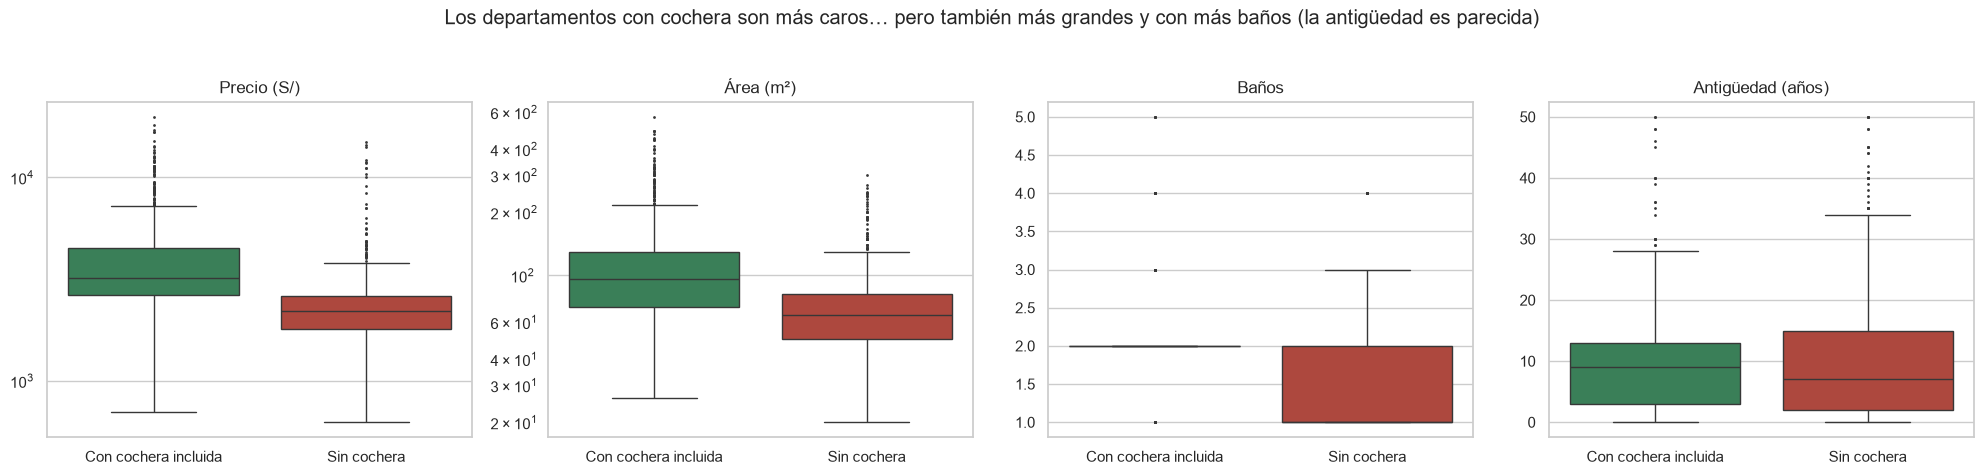
\includegraphics[width=\textwidth]{F0_eda_cochera_perfil.png}
\caption{Precio, área, baños y antigüedad de los avisos con y sin cochera incluida.}\label{fig:eda_perfil}
\origen{\texttt{notebook\_resumen.ipynb}, sección 2.2.}
\end{figure}

La cochera está repartida de forma muy desigual (figura~\ref{fig:coch_dist}): la incluye el 78\,\% de los avisos de Miraflores y el 68\,\% de los de San Isidro y Surco, frente al 20\,\% en San Miguel y el 15\,\% en Cercado. En los avisos que la cobran aparte, la mediana pedida es de \textbf{S/\,250 mensuales} (84 avisos en soles; rango intercuartil de S/\,200 a S/\,300). Es una referencia de mercado para la magnitud del efecto.

\begin{figure}[H]
\centering
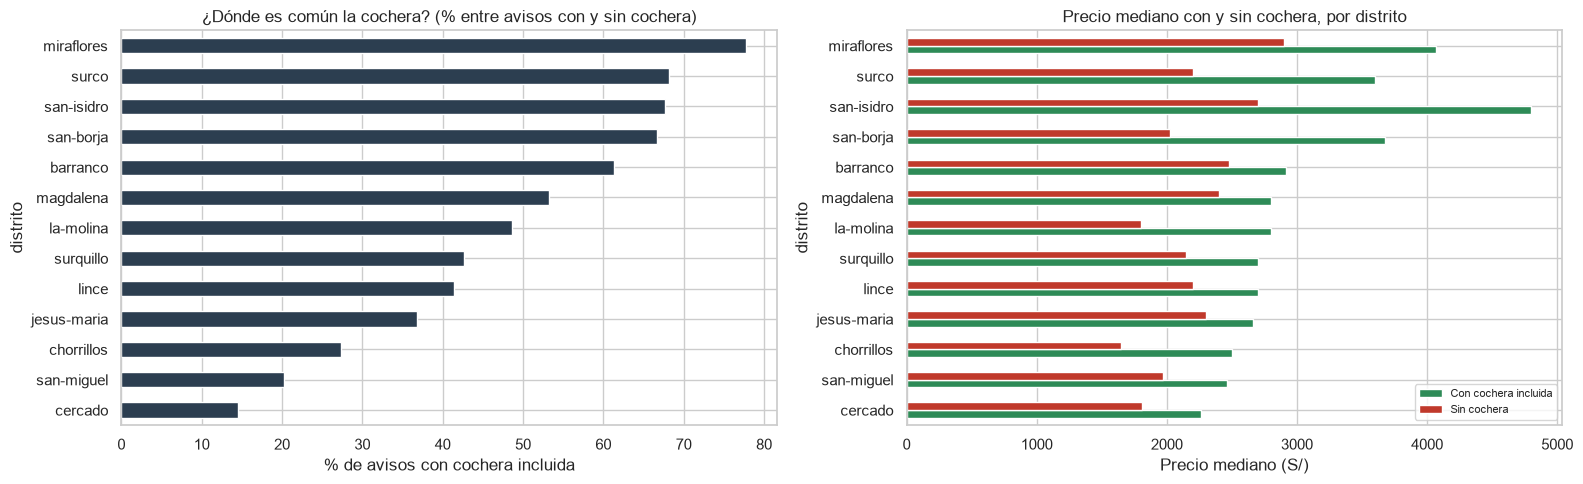
\includegraphics[width=\textwidth]{F0_eda_cochera_distrito.png}
\caption{Porcentaje de avisos con cochera incluida y alquiler mediano con y sin cochera, por distrito.}\label{fig:coch_dist}
\origen{\texttt{notebook\_resumen.ipynb}, sección 2.2.}
\end{figure}

\section{Soporte común y balance (R2)}\label{sec:res_soporte}

La propensión fuera de fold discrimina bien (AUC = 0.82; log-loss 0.52; Brier 0.17). Solo el 5\,\% de los avisos queda fuera de $[0.05,0.95]$, y el soporte común conserva 1\,949 avisos (1\,046 tratados y 903 controles). Antes de ponderar, las diferencias estandarizadas son grandes (0.92 en el área y 0.71 en los baños). Después, todas son menores que 0.05 en valor absoluto (figura~\ref{fig:soporte}): los grupos son comparables.

\begin{figure}[H]
\centering
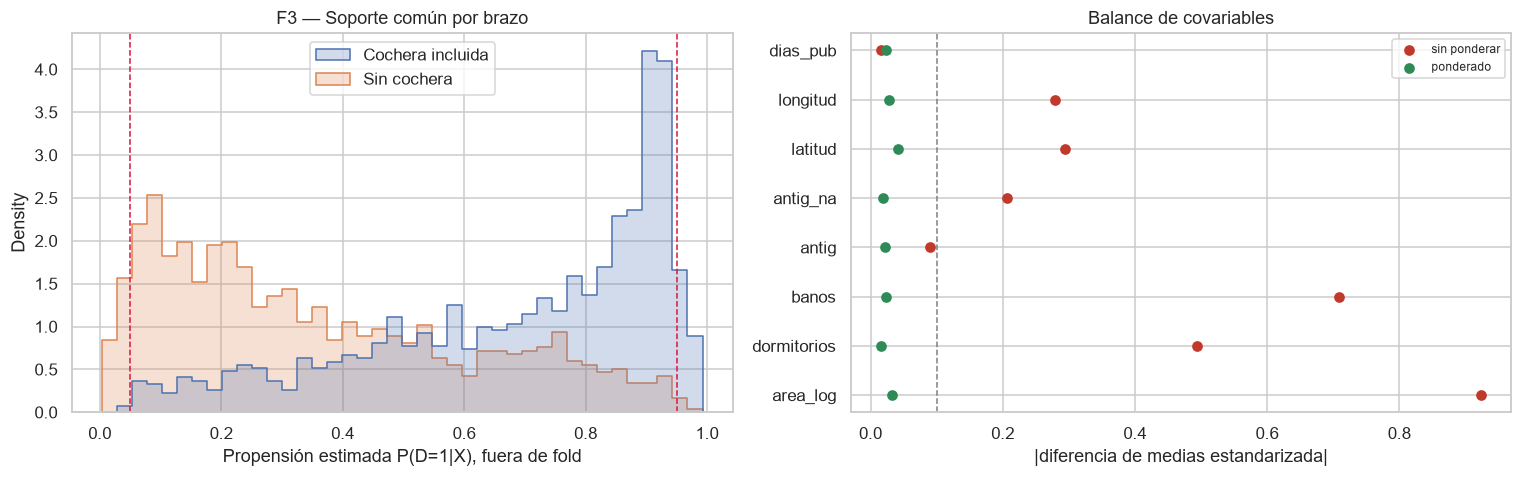
\includegraphics[width=0.95\textwidth]{F3_soporte_cochera.png}
\caption{Soporte común: propensión por grupo y balance antes y después de ponderar (R2).}\label{fig:soporte}
\origen{\texttt{notebook3b\_efecto\_cochera.ipynb}, sección 2 $\rightarrow$ \texttt{R2\_soporte.csv}, \texttt{R2\_balance.csv}.}
\end{figure}

\section{Efecto de la cochera incluida (R3)}\label{sec:res_efecto}

\begin{table}[H]
\centering\footnotesize
\caption{Efecto de tener cochera incluida sobre el precio de oferta (R3). EE agrupados por edificio}\label{tab:principal_c}
\resizebox{\textwidth}{!}{% Origen: notebook3b_efecto_cochera.ipynb -> resultados/tablas/R3c_principal.csv (generado por informe/tablas_manuscrito.py)
\begin{tabular}{lrrrcrcr}
\toprule
Estimador & N & $\theta$ & EE & IC 95\% ($\theta$) & \% efecto & IC 95\% (\%) & S/ al mes \\
\midrule
Diferencia sin ajustar (OLS) & 2,051 & 0.4883 & 0.0197 & [0.450, 0.527] & 63.0 & [56.8, 69.4] & 1,668 \\
Hedónico OLS & 2,051 & 0.0748 & 0.0133 & [0.049, 0.101] & 7.8 & [5.0, 10.6] & 206 \\
DML parcialmente lineal (PLR) & 2,051 & 0.0683 & 0.0119 & [0.045, 0.092] & 7.1 & [4.6, 9.6] & 187 \\
DML-IRM, muestra completa & 2,051 & 0.0425 & 0.0356 & [-0.027, 0.112] & 4.3 & [-2.7, 11.9] & 115 \\
DML-IRM, soporte común (principal) & 1,949 & 0.0724 & 0.0184 & [0.036, 0.108] & 7.5 & [3.7, 11.4] & 199 \\
\bottomrule
\end{tabular}}
\origen{\texttt{notebook3b\_efecto\_cochera.ipynb}, sección 3 $\rightarrow$ \texttt{R3c\_principal.csv}. Alquiler de referencia: S/\,2\,650.}
\end{table}

La diferencia bruta del 63\,\% se reduce, con el DML-IRM en el soporte común, a \textbf{7.5\,\% (IC 95\,\%: 3.7--11.4\,\%)}: unos \textbf{S/\,199 mensuales} (entre S/\,98 y S/\,303). El hedónico (7.8\,\%) y el PLR (7.1\,\%) coinciden. Sin recorte, el IRM es inestable (IC de $-2.7$ a 11.9\,\%), lo que confirma la necesidad del soporte común. Las 10 particiones dieron entre 6.8 y 9.4\,\%, y el modelo de precio explica el 82\,\% de la varianza fuera de fold. \textbf{H1 se confirma.}

\section{Grilla de especificaciones (R4)}\label{sec:res_grilla}

\begin{table}[H]
\centering\scriptsize
\caption{Efecto de la cochera bajo cada especificación (R4). DML-IRM, soporte común}\label{tab:especificaciones_c}
\resizebox{\textwidth}{!}{% Origen: notebook3b_efecto_cochera.ipynb -> resultados/tablas/R4c_especificaciones.csv (generado por informe/tablas_manuscrito.py)
\begin{tabular}{llp{3cm}rrrcr}
\toprule
Cód. & Especificación & Tipo & N & $\theta$ & EE & IC 95\% & \% efecto \\
\midrule
C1 & Principal & válida & 1,931 & 0.0732 & 0.0166 & [0.041, 0.106] & 7.6 \\
C2 & Sin área & omite confusor & 1,972 & 0.1081 & 0.0272 & [0.055, 0.161] & 11.4 \\
C3 & Sin ubicación (distrito, lat, lon) & omite confusor & 1,975 & 0.1961 & 0.0201 & [0.157, 0.236] & 21.7 \\
C4 & Sin baños ni dormitorios & omite confusor & 1,941 & 0.0868 & 0.0183 & [0.051, 0.123] & 9.1 \\
C5 & Sin antigüedad & omite confusor & 1,930 & 0.0775 & 0.0173 & [0.044, 0.111] & 8.1 \\
C6 & + precio/m$^2$ (descendiente de Y) & control inadmisible & 1,820 & -0.0046 & 0.0080 & [-0.020, 0.011] & -0.5 \\
C7 & Tratamiento estricto (incluida explícita) & medición & 547 & 0.0764 & 0.0342 & [0.009, 0.143] & 7.9 \\
C8 & Cochera con costo extra también como D=1 & medición & 2,113 & 0.0515 & 0.0156 & [0.021, 0.082] & 5.3 \\
C9 & + indicador de descripción cortada & medición & 1,926 & 0.0717 & 0.0181 & [0.036, 0.107] & 7.4 \\
P1 & Folds y EE por bloque de 1 km & partición & 1,953 & 0.0738 & 0.0204 & [0.034, 0.114] & 7.7 \\
\bottomrule
\end{tabular}}
\origen{\texttt{notebook3b\_efecto\_cochera.ipynb}, sección 4 $\rightarrow$ \texttt{R4c\_especificaciones.csv}.}
\end{table}

\begin{itemize}[itemsep=1pt]
\item \textbf{Confusores omitidos:} sin ubicación, el efecto casi se triplica (21.7\,\%), porque las cocheras abundan en las zonas caras. Sin área sube a 11.4\,\%.
\item \textbf{Control inadmisible:} el precio por m² lo anula ($-0.5$\,\%).
\item \textbf{Medición:} las alternativas se mueven en la dirección esperada. La definición estricta da 7.9\,\%, y contar las de costo extra como tratadas, 5.3\,\%.
\end{itemize}
El efecto se mueve mucho más con los controles que con el estimador (7.1--7.8\,\%). \textbf{H2 se confirma.}

\section{Robustez a confusores no observados (R5)}\label{sec:res_sens}

El valor de robustez es RV $=0.105$: un confusor que explique el 10.5\,\% de la variación residual de la cochera y del precio anularía el efecto. Para que el IC incluya el cero basta una fuerza de 0.054. Comparado con los observados (figura~\ref{fig:sensibilidad_c}), un confusor tan fuerte como la antigüedad llevaría el efecto a 0.4\,\%, y uno como la ubicación lo invertiría. La simulación muestra además que esta cota es optimista (sección~\ref{sec:res_sim}). El resultado es \textbf{frágil}. \textbf{H4 se confirma.}

\begin{figure}[H]
\centering
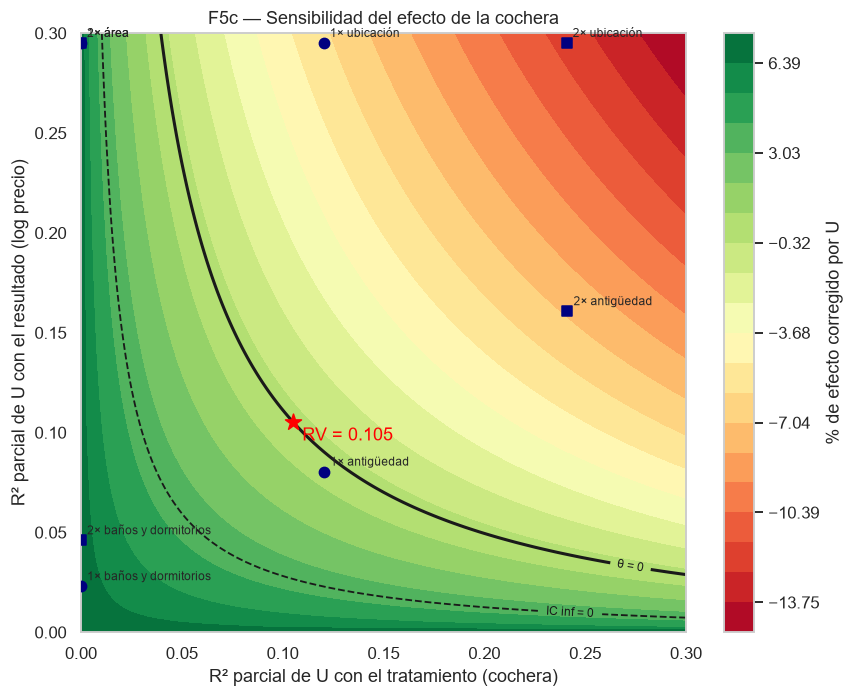
\includegraphics[width=0.6\textwidth]{F5c_sensibilidad_cochera.png}
\caption{Contorno de sensibilidad del efecto de la cochera con benchmarks observados (R5).}\label{fig:sensibilidad_c}
\origen{\texttt{notebook3b\_efecto\_cochera.ipynb}, sección 5 $\rightarrow$ \texttt{R5c\_sensibilidad.csv}.}
\end{figure}

\section{Heterogeneidad y dependencia espacial (R7)}\label{sec:res_het}

El efecto difiere por clase de distrito (figura~\ref{fig:gate_c}; Wald $\chi^2_2=18.3$, $p=0.0001$):
\begin{itemize}[itemsep=0pt]
\item \textbf{clase1} (Miraflores, San Isidro, Barranco, Lince): 1.5\,\%, con un IC que incluye el cero;
\item \textbf{clase2}: 10.3\,\%;
\item \textbf{clase3}: 17.8\,\%.
\end{itemize}
Por tamaño no hay diferencias ($p=0.35$). \textbf{H3 se confirma} por zona. Los residuos del precio tienen una autocorrelación espacial pequeña (I de Moran $=0.019$, $p=0.025$), y el IC agrupado por bloque de 1\,km también excluye el cero.

\begin{figure}[H]
\centering
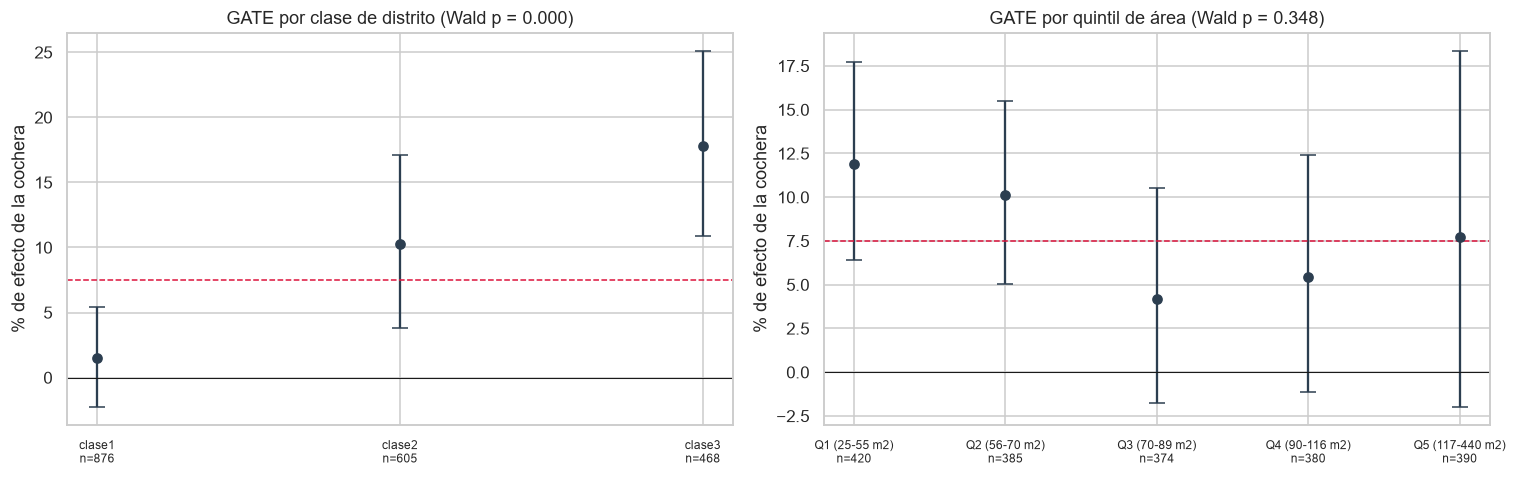
\includegraphics[width=\textwidth]{F7c_heterogeneidad_cochera.png}
\caption{Efecto de la cochera por clase de distrito y por quintil de área (R7).}\label{fig:gate_c}
\origen{\texttt{notebook3b\_efecto\_cochera.ipynb}, sección 6 $\rightarrow$ \texttt{R7c\_gate.csv}.}
\end{figure}

\section{Análisis secundario: un baño adicional}\label{sec:banos}

Con los mismos 2\,220 avisos (\texttt{notebook3\_estimacion\_causal}), la asociación bruta del 45.7\,\% se reduce a 7.4\,\% con el hedónico y a \textbf{3.8\,\% (IC 95\,\%: 1.7--6.0\,\%)} con el DML, unos S/\,100 mensuales:
\begin{itemize}[itemsep=0pt]
\item los \textit{learners} de árboles coinciden (3.8--4.4\,\%), mientras que Lasso, lineal, da 7.6\,\%;
\item sin área el efecto sube a 19.5\,\%, y con el precio por m² se anula;
\item agregar la cochera como control apenas lo cambia (3.5\,\%);
\item con todas las precisiones de geocodificación sube a 5.1\,\%: la ubicación imprecisa lo inflaba;
\item no hay heterogeneidad ($p>0.3$), y un confusor como la antigüedad lo dejaría en 0.7\,\% (RV = 0.079).
\end{itemize}

\section{Validación semisintética (R6)}\label{sec:res_sim}

\begin{table}[H]
\centering\small
\caption{Validación semisintética del estimador binario (100 réplicas por escenario; efecto verdadero 0.10)}\label{tab:sim_b}
\resizebox{0.85\textwidth}{!}{% Origen: notebook4_semisintetico.ipynb -> resultados/tablas/R6b_simulacion_binaria.csv (generado por informe/tablas_manuscrito.py)
\begin{tabular}{llrrrrr}
\toprule
Escenario & Estimador & $\theta$ verdadero & Sesgo & RMSE & Cobertura IC 95\% & Long. IC \\
\midrule
B1 & Hedónico OLS & 0.10 & 0.0002 & 0.0147 & 94 & 0.058 \\
B1 & DML PLR & 0.10 & -0.0040 & 0.0145 & 95 & 0.055 \\
B1 & DML-IRM (soporte común) & 0.10 & -0.0036 & 0.0198 & 96 & 0.081 \\
B2 & Hedónico OLS & 0.10 & 0.0412 & 0.0434 & 19 & 0.057 \\
B2 & DML PLR & 0.10 & 0.0392 & 0.0418 & 20 & 0.053 \\
B2 & DML-IRM (soporte común) & 0.10 & 0.0421 & 0.0462 & 45 & 0.078 \\
\bottomrule
\end{tabular}}
\origen{\texttt{notebook4\_semisintetico.ipynb} $\rightarrow$ \texttt{R6b\_simulacion\_binaria.csv}.}
\end{table}

\paragraph{Sin confusor omitido (B1).} Los tres estimadores recuperan el efecto: el sesgo es de 0.004 o menos y la cobertura del 94 al 96\,\%.

\paragraph{Con confusor moderado (B2).} Todos se sesgan ($\approx+0.04$) y la cobertura cae al 19--45\,\%. La cota de sensibilidad estimó un sesgo de 0.024 frente a uno real de 0.042, de modo que es \textbf{optimista} para el tratamiento binario.

\paragraph{Baños.} Para el estimador de baños, la simulación confirma tres cosas:
\begin{itemize}[itemsep=0pt]
\item sin confusor, el DML es insesgado (cobertura del 93\,\%), mientras que el hedónico lineal sobreestima el efecto (cobertura del 50\,\%);
\item con confusor, la cota sí es fiel (cobertura del 95--98\,\%);
\item la heterogeneidad real se detecta el 49\,\% de las veces.
\end{itemize}

\chapter{Discusión}\label{cap:discusion}

\section{Interpretación económica}

Entre departamentos publicados con dirección exacta y con igual área, dormitorios, baños, antigüedad y ubicación, los que incluyen cochera se ofrecen en promedio un 7.5\,\% más caros: unos S/\,199 al mes sobre un alquiler de S/\,2\,650, con un intervalo de S/\,98 a 303. Es una prima apreciable, pero muy lejana del 63\,\% de la comparación directa. Casi toda la diferencia bruta se explica porque los departamentos con cochera son más grandes y están en zonas más caras.

El hallazgo más interesante es la \textbf{heterogeneidad}. En los distritos de mayor precio (Miraflores, San Isidro, Barranco y Lince), la prima es casi nula (1.5\,\%), y crece al 10\,\% y al 18\,\% en las clases 2 y 3. Una explicación coherente con la teoría hedónica y con el contexto local es la escasez relativa. En Miraflores y San Isidro, la normativa municipal fija un número mínimo de estacionamientos por unidad de vivienda \citep{miraflores2011,sanisidro2020}. En la muestra, la mayoría de los avisos de esos distritos incluye cochera: el 78\,\% en Miraflores y el 68\,\% en San Isidro, frente al 15\,\% en Cercado y el 20\,\% en San Miguel (figura~\ref{fig:coch_dist}). Lince, también en la clase1, es una excepción (41\,\%). Donde la cochera es parte del estándar de la oferta comparable, no distingue a un aviso de otro y su precio implícito es bajo. Donde es escasa, el mercado la paga. Es una hipótesis explicativa, coherente con los datos, pero no contrastada formalmente aquí.

Tres cautelas: (i) es una prima sobre el precio \emph{de oferta}; (ii) se refiere a la población con soporte común y dirección exacta; y (iii) no es una recomendación de inversión. El efecto no dice si construir o asignar una cochera es rentable, porque no considera su costo.

\section{Comparación con los antecedentes}

\paragraph{Frente al propio avance previo.} El análisis exploratorio estimaba, con regresiones lineales por clase de distrito, que un baño adicional se asociaba con S/\,195--298 más de alquiler. El análisis causal sobre direcciones exactas lo reduce a unos S/\,100 (3.8\,\%). La diferencia se explica por el ajuste flexible de la confusión y por la calidad de la ubicación: con todas las precisiones de geocodificación el efecto sube a 5.1\,\%. La calidad de la geocodificación cambia el resultado y debe reportarse.

\paragraph{Frente a los estudios peruanos.} Los trabajos predictivos \citep{cacnahuaray2024,barrientos2026} identifican la cochera entre los determinantes más importantes del precio en Lima, y esta tesis lo confirma: el atributo importa. La diferencia está en qué se mide. Esos modelos cuantifican cuánto ayuda la cochera a \emph{predecir} el precio, una medida que mezcla su efecto con el del tamaño y la zona que la acompañan. Aquí se cuantifica cuánto cambia el precio por la cochera misma, y resulta mucho menos de lo que sugiere la asociación (7.5\,\% frente a 63\,\%). La grilla confirma además que la flexibilidad del DML no protege contra los malos controles \citep{hunermund2023}.

\citet{mundaca2018} no son comparables en magnitud con esta tesis, aunque coinciden en la dirección. Estudian precios de venta y el número de cocheras, mientras que esta tesis estudia el alquiler y la inclusión o no de la cochera. Ambos estudios coinciden en que la cochera es el atributo con mayor valoración y en que la ubicación es el principal confusor, que ellos señalan como su limitación.

\paragraph{Frente al propio mercado.} La comparación más directa en magnitud la ofrece la misma base de datos. Los avisos que cobran la cochera aparte piden una mediana de S/\,250 mensuales (sección~\ref{sec:res_ia}), del mismo orden que el efecto estimado de la cochera incluida (unos S/\,199). Que el efecto sea algo menor es razonable: el inquilino que la paga aparte la eligió porque la necesita.

\paragraph{Frente a la evidencia internacional.} \citet{gabbe2017} estiman que la cochera incluida eleva el alquiler en alrededor de 17\,\% en Estados Unidos. Que en Lima la prima sea menor (7.5\,\%) es coherente con una tenencia de automóviles mucho más baja, de alrededor del 17\,\% de los hogares \citep{limacomovamos2016}.

\section{Por qué el efecto podría estar sesgado}

\paragraph{Confusión no observada.} Un confusor tan fuerte como la antigüedad llevaría la prima de la cochera a cerca de cero, y la simulación muestra que la cota del estimador binario es optimista. El candidato natural es la \emph{calidad del edificio}: los proyectos de mayor estándar suelen incluir cochera y cobrar más por razones que el área y los baños no capturan del todo. La heterogeneidad atenúa en parte esta preocupación: si la prima fuera solo calidad omitida, cabría esperar que fuera mayor donde los edificios son de mayor estándar, y ocurre lo contrario.

\paragraph{Medición del tratamiento.} La clasificación depende del texto, y el 72\,\% de las descripciones termina con la marca ``Leer descripción completa''. Un aviso que no menciona su cochera queda como control. Si ese error es no diferencial, atenúa el efecto, y el valor real sería mayor. La especificación estricta (7.9\,\%) y la que controla por truncamiento (7.4\,\%) no sugieren un sesgo grande, pero la validación humana pendiente es la prueba que falta.

\paragraph{Selección por precisión de la dirección.} Las direcciones exactas son más caras y se concentran en los distritos caros. El efecto estimado no se transporta automáticamente a los avisos con dirección vaga.

\section{Amenazas a la validez y alcance}

\paragraph{Validez interna.} Persisten la confusión no observada, el error de medición del tratamiento y la autocorrelación espacial residual del precio. Esta última se trata con inferencia agrupada.

\paragraph{Validez externa.} La población es la de los avisos de un portal en 13 distritos, durante un mes y con dirección exacta. No se sabe si la prima de oferta se traslada al precio de contrato.

\paragraph{Validez de la medición con IA.} El modelo de lenguaje, con salida estructurada y temperatura 0, distinguió casos que una regex no puede (``no tiene cochera'', estacionamiento de visitas, costo aparte), y el piloto permitió corregir el prompt. Sin embargo, la guía metodológica exige una validación humana independiente antes de tratar la medición como confiable. Hasta entonces, los resultados de la cochera son exploratorios.

\section{Alcance de las aplicaciones}

El resultado sirve como referencia cuantitativa, con su incertidumbre y su fragilidad declaradas, para la tasación de alquileres y para entender cómo el mercado valora la cochera según la zona. No justifica afirmar que agregar una cochera elevará la renta en un 7.5\,\% en cualquier distrito, ni hacer recomendaciones sin considerar costos.

\chapter{Conclusiones y recomendaciones}\label{cap:conclusiones}

\section{Respuesta a la pregunta}

Entre avisos de alquiler de departamentos en 13 distritos de Lima con dirección exacta, y bajo el supuesto de que área, distribución, antigüedad y ubicación capturan lo que determina a la vez la cochera y el precio, \textbf{tener cochera incluida eleva el precio de oferta en 7.5\,\% (IC 95\,\%: 3.7--11.4\,\%), unos S/\,199 al mes}. La prima es casi nula donde la cochera es habitual y llega al 18\,\% donde escasea. El resultado es estable ante cambios de estimador y de definición del tratamiento, y sensible a los errores de especificación que advierte el DAG. Su fragilidad es considerable: un confusor tan influyente como la antigüedad bastaría para llevarlo cerca de cero.

\section{Conclusiones por objetivo}

\begin{table}[H]
\centering\small
\caption{Objetivo, evidencia y conclusión verificable}\label{tab:correspondencia}
\begin{tabularx}{\textwidth}{>{\raggedright\arraybackslash}p{2.4cm}>{\raggedright\arraybackslash}p{3.2cm}X}
\toprule
Objetivo & Evidencia & Conclusión \\
\midrule
OE1 Auditoría & Tabla~\ref{tab:exclusiones} & 2\,220 avisos válidos de 3\,739; 243 duplicados y 30\,\% de direcciones imprecisas detectados \\
OE2 Identificación & Figura~\ref{fig:dag}, tabla~\ref{tab:roles}, figura~\ref{fig:soporte} & Estimando defendible en el soporte común (95\,\% de la muestra, grupos balanceados); amenaza: calidad del edificio \\
OE3 Estimación & Tabla~\ref{tab:principal_c} & +7.5\,\% frente a 63\,\% bruto; los estimadores coinciden. \textbf{H1 se confirma} \\
OE4 Variación y sensibilidad & Tabla~\ref{tab:especificaciones_c}, figuras~\ref{fig:sensibilidad_c} y \ref{fig:gate_c} & Los controles importan más que el estimador (\textbf{H2}); efecto heterogéneo por zona (\textbf{H3}); frágil frente a confusores (\textbf{H4}) \\
OE5 Medición con IA & Tabla~\ref{tab:extraccion} & Medición barata (0.76 USD) y trazable; exploratoria hasta validarla \\
OE6 Validación & Tabla~\ref{tab:sim_b} & Los estimadores funcionan sin confusión omitida; la cota binaria es optimista \\
OE7 Trazabilidad & Anexo~\ref{anx:inventario} & Cada resultado es rastreable a su notebook; falta un comando único \\
\bottomrule
\end{tabularx}
\end{table}

\paragraph{Tres tipos de afirmaciones.}
\begin{itemize}[itemsep=1pt]
\item \textbf{Observacional:} los avisos con cochera cuestan un 63\,\% más, pero casi todo es tamaño y zona.
\item \textbf{Causal condicionada a los supuestos:} la cochera incluida eleva el alquiler de oferta entre 3.7 y 11.4\,\%, y más donde escasea.
\item \textbf{Hipótesis futuras:} que la heterogeneidad responda a la escasez y a la normativa, y que la prima de oferta se traslade al contrato.
\end{itemize}

\section{Límites del trabajo}\label{sec:limites}

\begin{itemize}[leftmargin=*,itemsep=1pt]
\item \textbf{Identificación:} la ignorabilidad solo puede acotarse, y la calidad del edificio no se observa.
\item \textbf{Medición:} la IA no tiene validación humana. Además, ``sin mención'' se trata como ``sin cochera'', y el 72\,\% de las descripciones podría estar truncado.
\item \textbf{Tratamiento:} es sí/no; las cocheras múltiples (26\,\% de los tratados) se agrupan y las de costo extra se excluyen.
\item \textbf{Sensibilidad:} la cota binaria es optimista.
\item \textbf{Población:} oferta, no contrato; un portal y un mes; solo direcciones exactas, que excluyen el 30\,\% de los avisos.
\end{itemize}

\section{Recomendaciones}

\begin{enumerate}[itemsep=1pt]
\item \textbf{Validar la medición} con los 249 avisos etiquetados a mano y corregir el efecto con el estimador de \citet{egami2023}.
\item \textbf{Medir la calidad del edificio} desde el texto (ascensor, acabados, seguridad) para reducir la amenaza principal.
\item \textbf{Ampliar los datos} a más meses y portales, y \textbf{consolidar el repositorio} con un comando único reproducible.
\end{enumerate}


\begin{thebibliography}{99}
\addcontentsline{toc}{chapter}{Referencias}
\setlength{\itemsep}{0.3em}

\bibitem[Advani et~al.(2019)]{advani2019}
Advani, A., Kitagawa, T., \& Słoczyński, T. (2019). Mostly harmless simulations? Using Monte Carlo studies for estimator selection. \textit{Journal of Applied Econometrics, 34}(6), 893--910. https://doi.org/10.1002/jae.2724

\bibitem[Athey et~al.(2019)]{athey2019}
Athey, S., Tibshirani, J., \& Wager, S. (2019). Generalized random forests. \textit{The Annals of Statistics, 47}(2), 1148--1178. https://doi.org/10.1214/18-AOS1709

\bibitem[Bach et~al.(2022)]{bach2022}
Bach, P., Chernozhukov, V., Kurz, M. S., \& Spindler, M. (2022). DoubleML: An object-oriented implementation of double machine learning in Python. \textit{Journal of Machine Learning Research, 23}(53), 1--6. https://www.jmlr.org/papers/v23/21-0862.html

\bibitem[Barrientos et~al.(2026)]{barrientos2026}
Barrientos, R., Delgado, R., Escalante, L., Febres, G., Hisbes, B., Chavez-Bedoya, L., Rosales, F., \& Vargas, W. (2026). Using machine learning to predict apartment prices in Lima. En \textit{Entrepreneurship and human-centric business strategies for social and economic resilience} (pp. 2725--2737). Springer. https://doi.org/10.1007/978-981-95-6415-6\_168

\bibitem[Boeing y Waddell(2017)]{boeing2017}
Boeing, G., \& Waddell, P. (2017). New insights into rental housing markets across the United States: Web scraping and analyzing Craigslist rental listings. \textit{Journal of Planning Education and Research, 37}(4), 457--476. https://doi.org/10.1177/0739456X16664789

\bibitem[Black(1999)]{black1999}
Black, S. E. (1999). Do better schools matter? Parental valuation of elementary education. \textit{The Quarterly Journal of Economics, 114}(2), 577--599. https://doi.org/10.1162/003355399556070

\bibitem[Cacñahuaray y Jiménez(2024)]{cacnahuaray2024}
Cacñahuaray Huaraca, J. C., \& Jiménez Novoa, S. M. (2024). \textit{Modelo predictivo de precios de alquiler de departamentos en la provincia de Lima usando técnicas de machine learning} [Tesis de segunda especialidad, Universidad Peruana Unión]. Repositorio institucional UPeU.

\bibitem[Cameron y Miller(2015)]{cameron2015}
Cameron, A. C., \& Miller, D. L. (2015). A practitioner's guide to cluster-robust inference. \textit{Journal of Human Resources, 50}(2), 317--372. https://doi.org/10.3368/jhr.50.2.317

\bibitem[Chay y Greenstone(2005)]{chay2005}
Chay, K. Y., \& Greenstone, M. (2005). Does air quality matter? Evidence from the housing market. \textit{Journal of Political Economy, 113}(2), 376--424. https://doi.org/10.1086/427462

\bibitem[Chen et~al.(2026)]{chen2026}
Chen, Z., Moeltner, K., \& Mair, M. (2026). \textit{Recovering direct price effects of environmental amenities in housing markets: Regression and causal machine learning model assessment with empirical Monte Carlo simulation} (arXiv:2606.02795). arXiv. https://arxiv.org/abs/2606.02795

\bibitem[Chernozhukov et~al.(2018)]{chernozhukov2018}
Chernozhukov, V., Chetverikov, D., Demirer, M., Duflo, E., Hansen, C., Newey, W., \& Robins, J. (2018). Double/debiased machine learning for treatment and structural parameters. \textit{The Econometrics Journal, 21}(1), C1--C68. https://doi.org/10.1111/ectj.12097

\bibitem[Chernozhukov et~al.(2022)]{chernozhukov2022}
Chernozhukov, V., Cinelli, C., Newey, W., Sharma, A., \& Syrgkanis, V. (2022). \textit{Long story short: Omitted variable bias in causal machine learning} (NBER Working Paper No. 30302). National Bureau of Economic Research. https://www.nber.org/papers/w30302

\bibitem[Cinelli et~al.(2024)]{cinelli2024}
Cinelli, C., Forney, A., \& Pearl, J. (2024). A crash course in good and bad controls. \textit{Sociological Methods \& Research, 53}(3), 1071--1104. https://doi.org/10.1177/00491241221099552

\bibitem[Cinelli y Hazlett(2020)]{cinelli2020}
Cinelli, C., \& Hazlett, C. (2020). Making sense of sensitivity: Extending omitted variable bias. \textit{Journal of the Royal Statistical Society: Series B, 82}(1), 39--67. https://doi.org/10.1111/rssb.12348

\bibitem[Contreras et~al.(2024)]{contreras2024}
Contreras, C., Aguilar, D., \& Lázaro, J. (2024). Impacto del transporte masivo en la informalidad de vivienda: el caso de la Línea 1 del Metro de Lima. \textit{Argumentos, 5}(1). Instituto de Estudios Peruanos. https://doi.org/10.46476/ra.v5i1.183

\bibitem[Egami et~al.(2023)]{egami2023}
Egami, N., Hinck, M., Stewart, B. M., \& Wei, H. (2023). Using imperfect surrogates for downstream inference: Design-based supervised learning for social science applications of large language models. En \textit{Advances in Neural Information Processing Systems 36} (NeurIPS 2023).

\bibitem[Faxvaag et~al.(2026)]{faxvaag2026}
Faxvaag, H., Aarsnes, U., \& Oust, A. (2026). Incorporating large language models in automated real estate valuation. \textit{Journal of Real Estate Research, 48}(3), 454--479. https://doi.org/10.1080/08965803.2025.2587313

\bibitem[Gabbe y Pierce(2017)]{gabbe2017}
Gabbe, C. J., \& Pierce, G. (2017). Hidden costs and deadweight losses: Bundled parking and residential rents in the metropolitan United States. \textit{Housing Policy Debate, 27}(2), 217--229. https://doi.org/10.1080/10511482.2016.1205647

\bibitem[Gyger et~al.(2026)]{gyger2026}
Gyger, T., Hauri, S., Bühlmann, S., Lehner, M., Schlesinger, J., \& Sigrist, F. (2026). Explainable spatial machine learning for hedonic real estate modeling. \textit{Real Estate Economics, 54}(3), 761--806. https://doi.org/10.1111/1540-6229.70030

\bibitem[Hernán y Robins(2020)]{hernan2020}
Hernán, M. A., \& Robins, J. M. (2020). \textit{Causal inference: What if}. Chapman \& Hall/CRC.

\bibitem[Hünermund et~al.(2023)]{hunermund2023}
Hünermund, P., Louw, B., \& Caspi, I. (2023). Double machine learning and automated confounder selection: A cautionary tale. \textit{Journal of Causal Inference, 11}(1), 20220078. https://doi.org/10.1515/jci-2022-0078

\bibitem[Imbens y Rubin(2015)]{imbens2015}
Imbens, G. W., \& Rubin, D. B. (2015). \textit{Causal inference for statistics, social, and biomedical sciences: An introduction}. Cambridge University Press.

\bibitem[Keele y Titiunik(2015)]{keele2015}
Keele, L. J., \& Titiunik, R. (2015). Geographic boundaries as regression discontinuities. \textit{Political Analysis, 23}(1), 127--155. https://doi.org/10.1093/pan/mpu014

\bibitem[Knaus et~al.(2021)]{knaus2021}
Knaus, M. C., Lechner, M., \& Strittmatter, A. (2021). Machine learning estimation of heterogeneous causal effects: Empirical Monte Carlo evidence. \textit{The Econometrics Journal, 24}(1), 134--161. https://doi.org/10.1093/ectj/utaa014

\bibitem[Lima Cómo Vamos(2016)]{limacomovamos2016}
Lima Cómo Vamos. (2016). \textit{Cómo vamos en movilidad: sexto informe de resultados sobre calidad de vida en Lima y Callao 2015}. Lima Cómo Vamos.

\bibitem[Manville(2013)]{manville2013}
Manville, M. (2013). Parking requirements and housing development: Regulation and reform in Los Angeles. \textit{Journal of the American Planning Association, 79}(1), 49--66. https://doi.org/10.1080/01944363.2013.785346

\bibitem[Mayo(2017)]{mayo2017}
Mayo Urtecho, H. M. (2017). \textit{Elaboración de un índice de precios de viviendas nuevas para Lima Metropolitana mediante precios hedónicos} [Tesis de grado, Universidad Nacional de Ingeniería]. http://hdl.handle.net/20.500.14076/13730

\bibitem[Municipalidad de Miraflores(2011)]{miraflores2011}
Municipalidad de Miraflores. (2011). \textit{Ordenanza N.° 342/MM: aprueban parámetros urbanísticos y edificatorios y las condiciones generales de edificación en el distrito} (art. 10: número mínimo de estacionamientos por unidad de vivienda; modificada por las Ordenanzas 385-MM y 466-MM).

\bibitem[Municipalidad de San Isidro(2020)]{sanisidro2020}
Municipalidad de San Isidro. (2020). \textit{Ordenanza N.° 523-MSI} (parámetros de estacionamiento para edificaciones multifamiliares).

\bibitem[Malpezzi(2003)]{malpezzi2003}
Malpezzi, S. (2003). Hedonic pricing models: A selective and applied review. En T. O'Sullivan \& K. Gibb (Eds.), \textit{Housing economics and public policy} (pp. 67--89). Blackwell.

\bibitem[Moran(1950)]{moran1950}
Moran, P. A. P. (1950). Notes on continuous stochastic phenomena. \textit{Biometrika, 37}(1/2), 17--23. https://doi.org/10.2307/2332142

\bibitem[Mundaca y Sánchez(2018)]{mundaca2018}
Mundaca, F., \& Sánchez, E. (2018). Índice de precios de inmuebles: un enfoque hedónico. \textit{Revista Estudios Económicos, 36}, 55--74. Banco Central de Reserva del Perú.

\bibitem[Nowak y Smith(2017)]{nowak2017}
Nowak, A., \& Smith, P. (2017). Textual analysis in real estate. \textit{Journal of Applied Econometrics, 32}(4), 896--918. https://doi.org/10.1002/jae.2550

\bibitem[Pearl(2009)]{pearl2009}
Pearl, J. (2009). \textit{Causality: Models, reasoning, and inference} (2.ª ed.). Cambridge University Press.

\bibitem[Pedregosa et~al.(2011)]{pedregosa2011}
Pedregosa, F., Varoquaux, G., Gramfort, A., Michel, V., Thirion, B., Grisel, O., et al. (2011). Scikit-learn: Machine learning in Python. \textit{Journal of Machine Learning Research, 12}, 2825--2830.

\bibitem[Rivera(2018)]{rivera2018}
Rivera Romero, L. A. (2018). \textit{Caso: determinantes del precio por metro cuadrado para departamentos en Lima Metropolitana: período 2005--2017} [Trabajo académico, Universidad de Lima].

\bibitem[Robinson(1988)]{robinson1988}
Robinson, P. M. (1988). Root-N-consistent semiparametric regression. \textit{Econometrica, 56}(4), 931--954. https://doi.org/10.2307/1912705

\bibitem[Rosen(1974)]{rosen1974}
Rosen, S. (1974). Hedonic prices and implicit markets: Product differentiation in pure competition. \textit{Journal of Political Economy, 82}(1), 34--55. https://doi.org/10.1086/260169

\bibitem[Shen y Ross(2021)]{shen2021}
Shen, L., \& Ross, S. (2021). Information value of property description: A machine learning approach. \textit{Journal of Urban Economics, 121}, 103299. https://doi.org/10.1016/j.jue.2020.103299

\bibitem[Sirmans et~al.(2005)]{sirmans2005}
Sirmans, G. S., Macpherson, D. A., \& Zietz, E. N. (2005). The composition of hedonic pricing models. \textit{Journal of Real Estate Literature, 13}(1), 1--44. https://doi.org/10.1080/10835547.2005.12090154

\bibitem[Tapia et~al.(2025)]{tapia2025}
Tapia, J., Chavez-Garzon, N., Pezoa, R., Suarez-Aldunate, P., \& Pilleux, M. (2025). Comparing automated valuation models for real estate assessment in the Santiago Metropolitan Region: A study on machine learning algorithms and hedonic pricing with spatial adjustments. \textit{PLOS ONE, 20}(3), e0318701. https://doi.org/10.1371/journal.pone.0318701

\bibitem[Urbania(2025)]{urbania2025}
Urbania. (2025). \textit{Urbania Index: índice de venta y alquiler, informe de mercado Lima, julio 2025}. https://urbania.pe/blog/urbania-index-lima/

\bibitem[VanderWeele y Ding(2017)]{vanderweele2017}
VanderWeele, T. J., \& Ding, P. (2017). Sensitivity analysis in observational research: Introducing the E-value. \textit{Annals of Internal Medicine, 167}(4), 268--274. https://doi.org/10.7326/M16-2607

\bibitem[Wager y Athey(2018)]{wager2018}
Wager, S., \& Athey, S. (2018). Estimation and inference of heterogeneous treatment effects using random forests. \textit{Journal of the American Statistical Association, 113}(523), 1228--1242. https://doi.org/10.1080/01621459.2017.1319839

\end{thebibliography}


\appendix
\chapter{Correspondencia con la rúbrica de evaluación}\label{anx:rubrica}

\begin{table}[H]
\centering\small
\begin{tabularx}{\textwidth}{>{\raggedright\arraybackslash}p{4.4cm}r>{\raggedright\arraybackslash}X}
\toprule
Criterio de la rúbrica & Puntos & Dónde se desarrolla \\
\midrule
Justificación científica & 2 & Sección~\ref{sec:justif} \\
Hipótesis, objetivos & 2 & Secciones~\ref{sec:pregunta}--\ref{sec:hipotesis} y tabla~\ref{tab:hipotesis} \\
Revisión de antecedentes teóricos y experimentales & 2 & Capítulo~\ref{cap:estado} (secciones~\ref{sec:ant_teo} y \ref{sec:ant_exp}) y anexo~\ref{anx:busqueda} \\
Presentación de resultados teóricos y/o experimentales & 4 & Teóricos: capítulos~\ref{cap:marco}--\ref{cap:diseno}. Experimentales: capítulo~\ref{cap:resultados} (tabla~\ref{tab:resumen_res}) \\
Discusión de resultados & 2 & Capítulo~\ref{cap:discusion} \\
Conclusiones & 2 & Capítulo~\ref{cap:conclusiones} (tabla~\ref{tab:correspondencia}) \\
Bibliografía & 1 & 44 referencias en APA 7, con DOI verificados en Crossref y todas citadas en el texto \\
\bottomrule
\end{tabularx}
\end{table}

\chapter{Registro de la búsqueda bibliográfica}\label{anx:busqueda}

\textbf{Fuentes:} Google Scholar, RePEc, arXiv, NBER, Crossref; repositorios peruanos (ALICIA-CONCYTEC, UNI, UPeU, ESAN, Universidad de Lima, Universidad del Pacífico, IEP), BCRP y normativa municipal. Los metadatos se verificaron el 21 y el 25 de octubre de 2026.

\textbf{Cadenas principales:}
\begin{itemize}[itemsep=0pt]
\item \path{("double machine learning" OR "causal forest") AND (housing OR rental OR hedonic)}
\item \path{"precio alquiler departamentos Lima" AND (hedónico OR "machine learning" OR estacionamiento OR cochera)}
\item \path{("inferencia causal" OR "diferencias en diferencias") AND vivienda AND (Lima OR Perú)}
\item \path{("bundled parking" OR "parking premium") AND rent}
\item \path{("large language model" OR GPT) AND ("real estate" OR housing) AND listing}
\end{itemize}

\textbf{Criterios:} se incluyeron estudios que estiman precios implícitos, predicen precios o identifican efectos de atributos de la vivienda, y los trabajos metodológicos usados directamente. Se excluyeron los estudios sin metadatos verificables y las versiones duplicadas, en cuyo caso se cita la versión publicada.

\chapter{Reproducibilidad y trazabilidad}\label{anx:inventario}

\begin{table}[H]
\centering\footnotesize
\begin{tabularx}{\textwidth}{>{\raggedright\arraybackslash}p{5cm}X}
\toprule
Artefacto (\path{notebooks/}) & Contenido \\
\midrule
\path{notebook2_auditoria} & R1: limpieza, duplicados, ROOFTOP; genera \path{csv/data_causal_base.csv} \\
\path{notebook2b_extraccion_ia} + \path{extraccion_ia.py} & R8: extracción de la cochera (regex + OpenAI, con caché) \\
\path{notebook3b_efecto_cochera} & R2--R5, R7: resultado principal \\
\path{notebook3_estimacion_causal} & Análisis secundario (baños) \\
\path{notebook4_semisintetico} + \path{semisintetico.py} & R6: validación semisintética \\
\path{notebook_resumen} & EDA resumido y recorrido de toda la tesis \\
\path{causal_utils.py} & Estimadores DML (PLR, IRM), GATE, sensibilidad, Moran \\
\path{informe/tablas_manuscrito.py} & Convierte los CSV de resultados en las tablas del informe \\
\bottomrule
\end{tabularx}
\end{table}

\textbf{Orden de ejecución:} \path{notebook2} $\rightarrow$ \path{2b} $\rightarrow$ \path{3b} $\rightarrow$ \path{3} $\rightarrow$ \path{4} $\rightarrow$ \path{notebook_resumen} $\rightarrow$ \path{tablas_manuscrito.py} $\rightarrow$ compilación. La semilla es \path{SEED = 42}. Una segunda ejecución completa reprodujo exactamente las 29 tablas y los resúmenes.

\textbf{Software:} Python 3.13, pandas 3.0, scikit-learn 1.9 \citep{pedregosa2011}, statsmodels 0.15 y \texttt{gpt-4.1-mini-2025-04-14}, con el prompt v2.

\textbf{Privacidad:} los datos (\path{data/}, \path{csv/}) y la clave (\path{.env}) no se versionan, y la base analítica no contiene descripciones, direcciones ni teléfonos.


\end{document}
